% For tips on writing the thesis, see http://www.tug.org/pracjourn/2008-1/mori/mori.pdf

% Two side to save paper
% openrigth means to put the chapter tittle on the right pages
\documentclass[12pt,letterpaper,twoside,openright]{book}
\usepackage[utf8x]{inputenc}
\usepackage[T1]{fontenc}
% Language support
\usepackage[english,spanish]{babel}

\usepackage[table,xcdraw]{xcolor}


\newenvironment{dedication}
{
   \cleardoublepage
   \thispagestyle{empty}
   \vspace*{\stretch{1}}
   \hfill\begin{minipage}[t]{0.66\textwidth}
   \raggedright
}%
{
   \end{minipage}
   \vspace*{\stretch{3}}
   \clearpage
}

\newenvironment{acreditation}
{
   \cleardoublepage
   \thispagestyle{empty}
   %\vspace*{\stretch{1}}
   
   %\raggedright
}%
{
   
   %\vspace*{\stretch{3}}
   \clearpage
}


\newenvironment{notetoeditor}
{
   \begin{tcolorbox}[title={Nota al editor},colback=yellow!5!white]
}%
{
   \end{tcolorbox}
}

\newcommand*{\captionsource}[2]{%
	\caption[{#1}]{%
		#1%
		\\\hspace{\linewidth}%
		\textbf{Source:} #2%
	}%
}

\setcounter{tocdepth}{4}
\setcounter{secnumdepth}{4}

\selectlanguage{english}
%\usepackage[spanish]{datetime}

% We define some strings that will use along
\def \thesiskeywords {facial expression recognition, label distribution learning, lightweight deep learning, vision transformer, EfficientFace, APViT, AffectNet}
\def \pdfauthor {David Valverde Garro}
\def \thesistitle{Enhancing label distribution generation for lightweight facial expression recognition with local-global features and transformer guidance}

% Custom-commands and definitions
% See this file for defining the keywords that will show up on the PDF file
\input{../packages}
% Glossary entries. Add terms with \newglossaryentry{label}{name=..., description=...}
% Add acronyms with \newacronym{label}{ACRONYM}{Full form}
% Reference in text: \gls{label}, \Gls{label}, \glspl{label}, or \acrshort{label}, \acrlong{label}, \acrfull{label}

% --- Acronyms ---
\newacronym{apvit}{APViT}{Attention Pooling Vision Transformer}
\newacronym{fer}{FER}{Facial Expression Recognition}
\newacronym{hci}{HCI}{Human-Computer Interaction}
\newacronym{dl}{DL}{Deep Learning}
\newacronym{cv}{CV}{Computer Vision}
\newacronym{cnn}{CNN}{Convolutional Neural Network}
\newacronym{flops}{FLOPs}{Floating Point Operations}
\newacronym{itw}{ITW}{In-the-Wild}
\newacronym{ldl}{LDL}{Label Distribution Learning}
\newacronym{ldg}{LDG}{Label Distribution Generator}
\newacronym{edl}{EDL}{Emotion Distribution Learning}
\newacronym{sll}{SLL}{Single-Label Learning}
\newacronym{mll}{MLL}{Multi-Label Learning}
\newacronym{vit}{ViT}{Vision Transformer}
\newacronym{mhsa}{MHSA}{Multi-Head Self-Attention}
\newacronym{nlp}{NLP}{Natural Language Processing}
\newacronym{sgd}{SGD}{Stochastic Gradient Descent}
\newacronym{lfe}{LFE}{Local-Feature Extractor}
\newacronym{csm}{CSM}{Channel-Spatial Modulator}
\newacronym{app}{APP}{Attentive Patch Pooling}
\newacronym{atp}{ATP}{Attentive Token Pooling}
\newacronym{gap}{GAP}{Global Average Pooling}
\newacronym{anova}{ANOVA}{Analysis of Variance}
\newacronym{cam}{CAM}{Class Activation Map}
\newacronym{mtcnn}{MTCNN}{Multi-Task Cascaded Convolutional Networks}
\newacronym{mldg}{M-LDG}{Modified Label Distribution Generator}

% --- Terms (domain-specific and key concepts) ---
\newglossaryentry{facial-expression-recognition}{
  name=facial expression recognition,
  description={A field within affective computing that seeks to detect human emotions based on facial expressions; FER systems provide automated solutions that analyze facial features to identify the emotion being conveyed, typically through a pipeline of preprocessing, feature extraction, and classification}
}
\newglossaryentry{affective-computing}{
  name=affective computing,
  description={A field of research concerned with systems that detect, understand, or replicate human emotions; facial expression recognition is one of its application areas}
}
\newglossaryentry{lightweight-fer}{
  name=lightweight FER,
  description={Facial expression recognition approaches designed for resource-constrained settings (e.g., mobile or edge devices), balancing accuracy with low parameter count and computational cost}
}
\newglossaryentry{edge-computing}{
  name=edge computing,
  description={Computing performed near the source of data (e.g., on devices or local servers) rather than in a central cloud, often requiring efficient models for real-time or offline use}
}
\newglossaryentry{self-attention}{
  name=self-attention,
  description={A mechanism that computes a representation of a sequence by relating each position to every other position via query-key-value operations; often refers to scaled dot-product attention as proposed by Vaswani et al., used in Transformers and Vision Transformers}
}
\newglossaryentry{multi-head-self-attention}{
  name=multi-head self-attention,
  description={An extension of self-attention that linearly projects the query, key, and value vectors once per attention head, computes self-attention for all heads in parallel, and combines the results; proposed by Vaswani et al. to learn information at different representation levels, and used in stacked layers of the Transformer encoder and decoder}
}
\newglossaryentry{transformer}{
  name=Transformer,
  description={A neural network architecture based on stacked self-attention layers, originally proposed for sequence transduction; uses an encoder-decoder structure, with the encoder used in Vision Transformers for image classification}
}
\newglossaryentry{patch-embedding}{
  name=patch embedding,
  description={In Vision Transformers, the representation obtained by splitting an image into patches, flattening them, and linearly projecting to a sequence of vectors used as input to the transformer encoder}
}
\newglossaryentry{discrete-emotions}{
  name=discrete emotion model,
  description={A theory that represents emotions as a fixed set of categories (e.g., the six basic emotions: anger, disgust, fear, happiness, sadness, surprise), often extended with neutral and contempt}
}
\newglossaryentry{in-the-wild}{
  name=in-the-wild (ITW),
  description={Referring to data or conditions that are not controlled in a laboratory: natural variation in pose, occlusion, illumination, and context; FER ITW denotes facial expression recognition on such unconstrained images or datasets}
}
\newglossaryentry{label-distribution-learning}{
  name=label distribution learning,
  description={A learning paradigm where the target is a distribution over labels (e.g., description degrees per class) rather than a single label; a lightweight network may learn from soft distributions produced by a stronger model or a label distribution generator}
}
\newglossaryentry{emotion-distribution}{
  name=emotion distribution,
  description={A vector of description degrees (intensity values per emotion class), one per emotion class, that sum to one; used in emotion distribution learning to represent the intensity of each emotion in a facial expression}
}
\newglossaryentry{efficientface}{
  name=EfficientFace,
  description={A lightweight facial expression recognition network proposed by Zhao et al., built on ShuffleNet V2 with local-global feature extraction modules and trained via label distribution learning using a label distribution generator}
}
\newglossaryentry{label-distribution-generator}{
  name=label distribution generator,
  description={A network that produces soft label (emotion) distributions for training images; typically trained first and then used to generate targets for training a lightweight network, and can be discarded at inference}
}
\newglossaryentry{local-global-features}{
  name=local-global feature extraction,
  description={An architectural strategy that captures both local details (e.g., fine-grained facial regions) and global context (e.g., overall expression)}
}
\newglossaryentry{residual-connection}{
  name=residual connection,
  description={A skip connection that adds the input of a block to its output, enabling training of very deep networks by easing gradient flow; used e.g. in ResNets}
}
\newglossaryentry{knowledge-distillation}{
  name=knowledge distillation,
  description={Training a smaller or more efficient model to mimic the outputs of a larger or more accurate model, so that the former learns from the latter's soft predictions}
}
\newglossaryentry{retinaface}{
  name=RetinaFace,
  description={A face detection and alignment method that preprocesses facial images, ensuring consistent pose and landmark alignment}
}
\newglossaryentry{affectnet}{
  name=AffectNet,
  description={Large-scale in-the-wild facial expression dataset (approximately 1 million images) with 7 and 8-class subsets, widely used for training and evaluating FER models}
}
\newglossaryentry{static-fer}{
  name=static FER,
  description={Facial expression recognition on single images using only spatial information, as opposed to dynamic FER which uses video or image sequences}
}


\newtoggle{paper}
\settoggle{paper}{true}

\usepackage{csvsimple}


\begin{document}

% This is the first part of the document (frontmatter), use Roman numeration
\frontmatter

% Simple style
\pagestyle{empty}

% The front page of the thesis is in this page, Name of the school and the program can be changed here. Supervisor name gets changed here.
\selectlanguage{english}
\input{body/front-page}

%

\selectlanguage{spanish}
%\begin{acreditation}
% The ghesis act goes here.
%\makebox[\linewidth]{
    
\includegraphics[width=0.75\paperwidth,height=1\paperheight]{../images/certificate.pdf}
%}

%\end{acreditation}


\begin{dedication}
\selectlanguage{english}
I dedicate this work to my mother, who gave me this life and education, and to my father, who watches over me from the next one and inspired me to be an academic and professional.
\HRule\\
\selectlanguage{spanish}
Dedicado a mi madre, quien me dio esta vida y educación, y a mi padre, quien me observa desde la siguiente y me inspiró a ser académico y profesional.
\selectlanguage{english}
\end{dedication}

%%%%%%%%%ISSUE NUMBER 1%%%%%%%%%%%
\chapter*{Acknowledgements}
\doublespacing

I would like to express my sincere gratitude to Prof. Luis Alexander Calvo Valverde, my thesis advisor, for guiding this work with patience and wisdom.\\

I thank the members of the reader committee for the valuable time taken to review and consider this work.\\

I also thank the authors of the EfficientFace and APViT networks, as well as the authors of the AffectNet dataset for making their work available to the public. Their open-source implementations and datasets made reproducible experimentation possible.\\

Finally, I thank my friends and loved ones for their patience, encouragement, and friendly banter throughout this process.

% The abstract is included on a separte file here
\doublespacing

\selectlanguage{english}%
\begin{abstract}
\iftoggle{paper}
{
Lightweight facial expression recognition (FER) models are essential for resource-constrained deployment, yet they typically lag behind heavier transformer-based approaches in accuracy.
This thesis investigates whether enhancing the label distribution generator (LDG) used to train EfficientFace, a 1.28-million-parameter lightweight FER network, can close that accuracy gap without increasing the deployed model's cost.
Three LDG enhancements are evaluated: FER-pretrained APViT backbone weights, EfficientFace local-global feature modules, and label distribution learning guided by APViT outputs.
The study follows a two-phase factorial design on the AffectNet dataset (7- and 8-class subsets).

Phase I ablates the three enhancements on the modified LDG (M-LDG). APViT transformer guidance proved the only statistically significant factor, lifting M-LDG accuracy by 7.889 percentage points to 64.34\% on AffectNet-7 and 57.71\% on AffectNet-8. FER-pretrained weights and local-global modules contributed negligibly, due to mismatch with the M-LDG's deeper ResNet-50 backbone. Phase II trains two EfficientFace variants, one guided by the best M-LDG and one directly by APViT, and compares them against the published EfficientFace baseline.

The main hypothesis is rejected: neither variant surpassed the published baseline of 63.70\% on AffectNet-7 and 59.89\% on AffectNet-8. The best result, M-LDG-guided EfficientFace, reached 63.00\% and 55.99\% on the two subsets. A capacity bottleneck is identified: a parameter ratio of approximately 44:1 between M-LDG and EfficientFace is too wide for label distribution learning to bridge, unlike the modest gap in the original EfficientFace paper. Replacing the M-LDG with APViT as the direct teacher produced no statistically significant difference in student accuracy, suggesting that at this capacity scale the choice of teacher is secondary to the structural gap. Future work should address the bottleneck directly, for example through intermediate-capacity assistant networks or distribution sharpening techniques.
}%


\end{abstract}

\selectlanguage{english}


%Table of contents is generated here
\tableofcontents

%List of figures goes here
\listoffigures

%List of tables is generated here
\listoftables

\glsaddall
%\printglossary[type=\acronymtype, title=Glossary, toctitle=Glossary]
\printglossary


\mainmatter
% Use double space
\doublespacing
% Now fancy style
\pagestyle{fancy}
\setlength{\headheight}{14.5pt}
% Left the right header clean
\rhead{}

\renewcommand{\chaptername}{Chapter}

\doublespacing

% The section introduction is included
\chapter{Introduction}
\label{chapter:introduction}


\epigraph{``This can be used as an introductory quote''}{Quote author}

\newpage

Facial expression recognition (FER) plays a crucial role within human-computer interaction (HCI), enabling automated detection of human emotions from facial data \cite{li2022survey}.
FER has also attracted researchers in the field of affective computing, due to its potential applications in creating systems that detect, understand, and replicate emotions \cite{karnati2023survey}.
Thanks to advancements in computer vision and deep learning (DL) methods, FER technology has improved significantly over the recent years \cite{li2022survey}.
This thesis focuses on the subfield of lightweight FER for deployment on resource-constrained environments, which demands a balance between accuracy and efficiency.\\

FER systems have a wide range of applications, including sociable robots, medical treatment, driver safety, marketing, education, psychological research, and security \cite{li2022survey, karnati2023survey, canal2022survey, sajjad2023survey}.
Despite this, FER faces several challenges such as occlusion, pose and lighting conditions, subject variability, data annotation, resolution, among others \cite{li2022survey, sajjad2023survey}.
On top of this, real-world usage scenarios such as edge computing require the highest level of efficiency in order to be feasible \cite{wu2020edge}.\\

Given the proliferation of mobile and edge platforms with a limited resource budget, there is an increasing need for lightweight FER models.
Recent studies have focused on creating optimized deep learning methods for computer vision \cite{howard2017mobilenet, zhang2018shufflenet}, with some even applying such methods directly to FER \cite{eff-face2021, lengwe2023pattlite}.
These studies have shown that it is possible to significantly optimize these models while maintaining or even improving the system's accuracy.\\

This thesis aims to enhance the lightweight FER network, EfficientFace \cite{eff-face2021}, in order to improve its accuracy while maintaining its low resource cost.
To this end, we modify the authors' training approach by leveraging the APViT \cite{apvit2023} model, which achieves state-of-the-art results in FER.

\newpage

\section{Problem}

Facial expression recognition (FER) systems provide automated solutions that analyze facial features to identify the emotion being conveyed. 
In the context of static or image-based FER, feature-extracting CNNs followed by fully-connected  classifiers have been the generally predominant approach \cite{canal2022survey}.
Following the wider trend in deep computer vision, networks with self-attention mechanisms have been applied to the FER task to obtain significant classification improvements \cite{apvit2023, lengwe2023pattlite, xue2021transfer, ma2023asf, huang2021, pecoraro2022lhc}.
In particular, Vision Transformers are quite adept at the FER task when training with challenging pose, lighting and occlusion conditions (in-the-wild).
This is, in part, thanks to the network's ability to pay greater attention to more important facial regions, which mitigates the effect of occlusion and pose variations \cite{karnati2023survey}.\\

While several of these approaches have achieved state-of-the-art results, many of them incur a heavy resource cost in terms of network parameters and floating point operations per-second (FLOPs).
When considering that the feature extraction step is the system's bottleneck \cite{karnati2023survey}, these solutions can become unsuitable for resource-constrained environments.
Some FER researchers have developed lightweight approaches that aim to maintain a comparable level of performance while greatly reducing parameters and computational cost \cite{eff-face2021, lengwe2023pattlite, hewitt2018, mitre2020, barros2020fc}.
These proposals generally employ well-studied, lightweight CNN architectures and combine them with custom modules or training strategies to maintain robustness for FER ITW.
Such methods have achieved great results, with some even setting the current state-of-the-art \cite{lengwe2023pattlite}.
However, this is still only a small subset of FER research, and only an even smaller subset has been tested on ITW databases \cite{eff-face2021}.\\

One such lightweight FER network is EfficientFace \cite{eff-face2021}.
This network achieves great accuracy results on the RAF-DB (88.36\%) and AffectNet (63.7\%) datasets when taking into account its very low parameter count of 1.28 million.
However, other Transformer models like APViT \cite{apvit2023} are capable of achieving much better results (RAF-DB 91.98\%, AffectNet 66.91\%), albeit with a significant increase in computational cost (65.2 M parameters).

\section{Document Structure}
\textbf{TO-DO al finalizar el documento}

%Provide a brief explanation of the intent of this document, as well as what has been described in the current section. Then describe what is included in each one of the sections. An example is provided but should be changed by the author.

%\nameref{chapter:theoretical-framework} chapter brings the theoretical concepts needed for understanding the research developed in this thesis, as well as the related work describing the state of the art of the specific topic that the author worked on.
%The sections mentioned here are incomplete and should be completed with the specific chapters of the author.
%\nameref{chapter:hypothesis-objectives} describes the hypothesis defined for the research as well as a description of the objectives and its deliverables. Also, the scope and limitations of this research effort can be found in that chapter.

%\nameref{chapter:methodology} chapter describes the experiment executed for this thesis, including the experiment design, the hardware used, and the analysis method for the data obtained.

%The \nameref{chapter:design} chapter presents the selected state of the implementation of what the author developed in its document. Also, the design and implementation details of the developed work are presented in this chapter. 

%\nameref{chapter:results} displays the results of the data obtained through the experiment and, the  \nameref{chapter:discussion} chapter analyses all the information obtained in \nameref{chapter:results}.

%Finally, \nameref{chapter:conclusions-fw} shows all the obtained conclusions and remarks from the research presented in this document. Future work is identified in this chapter.
% Theoretical framework contents
\input{body/theoretical-framework}
% Hypothesis and objetives.
\chapter{Hypothesis and Objectives}
\label{chapter:hypothesis-objectives}
\epigraph{``The first principle is that you must not fool yourself --- and you are the easiest person to fool.''}{\vspace{10pt}Richard P. Feynman}

\newpage


\section{Hypothesis}
\label{section:hypothesis}
Based on the literature review and objectives of this research project, we present the following hypothesis:

\textit{``Training EfficientFace with a label distribution generator enhanced with one or more of: FER pretrained backbone weights, local-global feature extraction modules, and/or vision transformer guidance, should increase its facial expression recognition accuracy on the AffectNet dataset when compared to the original baseline''.}

\section{Objectives}
\label{section:objectives}
This section defines the main and specific objectives of our research proposal.\\
These objectives align with the complete execution of our proposed study.

\subsection{Main Objective}
\label{section:main-objective}
Based on our proposal to address the previously presented problem, we determine the main objective of our research project to be as follows:

\textit{Study the facial expression recognition accuracy obtained when training EfficientFace \cite{eff-face2021} with a label distribution generator enhanced with local-global feature extraction modules and knowledge from a vision transformer model \cite{apvit2023}. }

\subsection{Specific Objectives}
\label{section:specific-objectives}
In order to successfully complete our general objective, we derive the following specific objectives:

\begin{enumerate}
    \item Enhance the label distribution generator (LDG) by loading the pretrained weights from APViT's backbone, adding local-global feature extraction modules from EfficientFace, and training the LDG to imitate APViT's outputs using label distribution learning.

    \item Study the performance changes induced by each modification to the LDG by means of ablation study and determine the best combination.
    
    \item Train two EfficientFace variants, one using the modified LDG and one using APViT, and study the performance differences with respect to the baseline and other state-of-the-art approaches.
    
\end{enumerate}

\subsection{Deliverables}
This section defines the deliverables aligned with each of the specific objectives of the thesis study.

\textbf{Specific Objective 1:}
\begin{itemize}
    \item Python script that defines the modified LDG network architecture and its training procedure.
    \item Preprocessed AffectNet dataset.
\end{itemize}

\textbf{Specific Objective 2:}
\begin{itemize}
    \item Jupyter notebooks that automate the Phase I experiment execution.
    \item Raw data results from the Phase I experimental design execution.
    \item Raw data results from the Phase I hyperparameter optimization procedure.
    \item Trained weights of the resulting models.
\end{itemize}

\textbf{Specific Objective 3:}
\begin{itemize}
    \item Jupyter notebooks that automate the Phase II experiment execution.
    \item Raw data results from the Phase II experimental design execution.
    \item Raw data results from the Phase II hyperparameter optimization procedure.
    \item Trained weights of the resulting models.
\end{itemize}

\section{Scope and Limitations}\label{section:scope-limitations}

The following section outlines the scope and limitations of this research project. These are the specific boundaries set for the study, which limit the scope and define the operational framework within which the research was conducted. 

\begin{itemize} 

\item This research focuses exclusively on the static facial expression recognition task with images annotated under the 7 or 8 class discrete model.

\item This project does not extend to adjacent research areas such as facial detection, facial identification, dynamic (video) FER, micro-expression recognition, or FER with facial action units.

\item The preprocessing steps for the input images was carried out as outlined by the authors of EfficientFace and APViT in their respective papers \cite{eff-face2021, apvit2023}.

\item The materials used in this research are limited to publicly available resources. This includes datasets, research papers, source code, programming languages,  packages, and other language extensions.

\item Only deep learning methods for facial expression recognition were considered for the state-of-the-art comparison.

\end{itemize}
% Methodology
\chapter{Methodology}
\label{chapter:methodology}
\epigraph{``If you cannot measure it, you cannot improve it.''}{\vspace{10pt}Lord Kelvin }

\newpage

In this chapter we describe the key aspects of the methodology used to test our hypothesis and proposal.\\
We go over the two phase design of the study, along with their factors, levels, responses, inputs, statistical analysis and more.

\section{Experimental design}
\label{section:experiment-design}
The experimental design of this study is divided into two distinct phases to ensure a rigorous and replicable process. This division allows for a more thorough evaluation of the proposed modifications and a reduction in overall training time. The design for each of the phases follows the guidelines defined by Montgomery \cite{montgomery2017design}.

\subsection{Phase I: LDG ablation study}
The first phase focuses on analyzing the performance changes induced by modifying the label distribution generator (LDG) network that guides EfficientFace's training. An ablation study is conducted to evaluate the effects of each proposed modification to the LDG, concentrating solely on the accuracy response for the facial expression recognition (FER) task. EfficientFace is not trained or evaluated in this phase. The best modified LDG configuration identified here will be used in phase II.

\subsection{Phase II: EfficientFace training study}
The second phase analyzes the effectiveness of using the modified LDG as an intermediary to transfer knowledge from APViT to EfficientFace. The best LDG configuration from phase I is used to train EfficientFace, following the original procedure \cite{eff-face2021}. Additionally, an alternative EfficientFace variant is trained using APViT directly as its label distribution generator, skipping the modified LDG. A comparative experiment is conducted to determine the best approach.

\section{Factors and levels}
The factors and levels for each phase of the experimental design are summarized below.

\subsection{Phase I: LDG Ablation study}
The design factors for this phase are the three proposed modifications to the LDG (pretrained weights, local-global feature extraction, and transformer guidance), as well as the training dataset. Since this is an ablation study, the levels of the factors are binary (present or not present). The factors and levels are summarized in Table~\ref{tab:p1-factors}.

% Please add the following required packages to your document preamble:
% \usepackage{booktabs}
% \usepackage{multirow}
\begin{table}[h]
\centering
\begin{tabular}{@{}ccccc@{}}
\toprule
                                 & \multicolumn{4}{c}{\textbf{Factors}} \\
 &
  \begin{tabular}[c]{@{}c@{}}Pretrained \\ Weights\end{tabular} &
  \begin{tabular}[c]{@{}c@{}}GL Feature \\ Extraction\end{tabular} &
  \begin{tabular}[c]{@{}c@{}}Transformer\\ Guidance\end{tabular} &
  Dataset \\ \midrule
\multirow{2}{*}{\textbf{Levels}} & Yes    & Yes   & Yes   & AffectNet (7 class)      \\
                                 & No     & No    & No    & AffectNet (8 class)   \\ \bottomrule
\end{tabular}
\caption{Factors and levels of phase I}
\label{tab:p1-factors}
\end{table}

\subsection{Phase II: EfficientFace training study}
The design factors for this phase are the guidance network (modified LDG or APViT) and the dataset (AffectNet 7-class or 8-class subset). The factors and levels are summarized in Table~\ref{tab:p2-factors}.

% Please add the following required packages to your document preamble:
% \usepackage{multirow}
\begin{table}[h]
\centering
\begin{tabular}{clcc}
\hline
                                 &  & \multicolumn{2}{c}{\textbf{Factors}}                                   \\
                                 &  & \begin{tabular}[c]{@{}c@{}}Guidance\\ Net\end{tabular} & Dataset   \\ \hline
\multirow{2}{*}{\textbf{Levels}} &  & M-LDG                                                      & AffectNet (7 class)    \\
                                 &  & APViT                                                      & AffectNet (8 class) \\ \hline
\end{tabular}
\caption{Factors and levels of phase II}
\label{tab:p2-factors}
\end{table}

\section{Measures and combinations of the experiment}
The measures and treatment combinations for each phase are described below.

\subsection{Phase I: LDG ablation study}
A $2^k$ factorial design with $k=4$ is used to explore the effects of each LDG modification and their interactions, with both AffectNet subsets. This results in 8 treatment combinations per subset, for a total of 16 experimental runs. The treatment combinations are shown in Table~\ref{tab:p1-runs}.\\
For reference, the factors are pretrained weights (A), GL feature extraction modules (B), APViT guidance (C), and dataset (D).

% Please add the following required packages to your document preamble:
% \usepackage{booktabs}
\begin{table}[h]
\centering
\begin{tabular}{@{}clccclcc@{}}
\toprule
\textbf{Run} &  & \textbf{A} & \textbf{B} & \textbf{C} & \textbf{D} &  & \textbf{Label} \\ \midrule
0  &  &  +  &  +  &  +  &     &  & abc   \\
1  &  &  +  &  +  &  +  &  +  &  & abcd  \\
2  &  &  +  &  +  &     &     &  & ab    \\
3  &  &  +  &  +  &     &  +  &  & abd   \\
4  &  &  +  &     &  +  &     &  & ac    \\
5  &  &  +  &     &  +  &  +  &  & acd   \\
6  &  &  +  &     &     &     &  & a     \\
7  &  &  +  &     &     &  +  &  & ad    \\
8  &  &     &  +  &  +  &     &  & bc    \\
9  &  &     &  +  &  +  &  +  &  & bcd   \\
10 &  &     &  +  &     &     &  & b     \\
11 &  &     &  +  &     &  +  &  & bd    \\
12 &  &     &     &  +  &     &  & c     \\
13 &  &     &     &  +  &  +  &  & cd    \\
14 &  &     &     &     &     &  & (1)   \\
15 &  &     &     &     &  +  &  & d     \\ \bottomrule
\end{tabular}
\caption{Treatment combinations for phase I.}
\label{tab:p1-runs}
\end{table}

\subsection{Phase II: EfficientFace training study}
A $2^k$ factorial design with $k=2$ is used, resulting in 4 treatment combinations executed in randomized order. Additional runs may be added based on hyperparameter variation. The treatment combinations are shown in Table~\ref{tab:p2-runs}.\\
The factors in this phase are labeled: guidance network (G), and dataset (D).

% Please add the following required packages to your document preamble:
% \usepackage{booktabs}
\begin{table}[h]
\centering
\begin{tabular}{@{}cccc@{}}
\toprule
\textbf{Run} &  & \textbf{G} & \textbf{D} \\ \midrule
1            &  & LDG        & AffectNet (7 class)     \\
2            &  & LDG      & AffectNet (8 class)     \\
3            &  & APViT        & AffectNet (7 class)  \\
4            &  & APViT      & AffectNet (8 class) \\ \bottomrule
\end{tabular}
\caption{Treatment combinations for phase II}
\label{tab:p2-runs}
\end{table}

\section{Response variable}
For both phases of this study, the top-1 accuracy metric obtained on the evaluation or test set after executing the full training procedure is taken as the sole response variable. This aligns with common practice in FER studies, where accuracy is the main metric for comparison with other approaches \cite{li2022survey, karnati2023survey, canal2022survey}.\\
Top-1 accuracy measures the fraction of samples where the model's most confident prediction exactly matches the true label:\\
\begin{equation}
    \text{Top-1 Accuracy} = \frac{1}{N} \sum_{i=1}^{N} \left[ y_i = \hat{y}_i \right]\\
\end{equation}
where $N$ is the total number of samples, $y_i$ is the true label, and $\hat{y}_i$ is the predicted label with the highest probability.

\section{Experiment set up and data collection}
The execution of the experiments in both phases is facilitated by Jupyter notebooks that automate set up and parameterization.\\
For each phase there are $n=2^k$ notebooks, each with the correct treatment combinations according to tables \ref{tab:p1-runs} and \ref{tab:p2-runs}.\\
The notebook uses the levels to download the correct dataset, pretrained weights, and training script.\\
The script is then executed using the levels corresponding to the actual combination.\\

The randomization of runs and execution of the actual notebook is manually performed in the execution environment.\\
Multiple VastAI instances with a single Nvidia RTX 3090 GPU were used as the execution environment, isolating each run in its own instance.\\
The data collection is also automated via Wandb integration in the training scripts.\\
All experimental runs are logged to this service, registering accuracy, loss, confusion matrices, and hyperparameters, among other data.

\section{Description of the inputs of the system}
The main inputs to the system are the AffectNet dataset and the network weights for APViT and EfficientFace. All images are preprocessed using RetinaFace \cite{retinaface2020} for face alignment and maintaining the pipeline used in the original scripts of APViT \cite{apvit2023} and EfficientFace \cite{eff-face2021}.

\section{Statistical tool}
To analyze the results of both experimental phases, we use analysis of variance (ANOVA) to determine if there are statistically significant differences between the treatment combinations. The procedure is as follows:\\

First, we check the assumptions required for ANOVA, such as normality of residuals and homogeneity of variance, using diagnostic plots and statistical tests. If the assumptions are not met, appropriate data transformations or non-parametric alternatives are considered.\\

For Phase I, after estimating the effects of each factor, negligible factors are discarded to focus the analysis on the most relevant variables. This also has the advantage of effectively adding replications to the remaining factor combinations, improving the reliability of the results. In Phase II, all factors are retained since multiple replications are available for each combination.\\

Descriptive statistics and visualizations, such as boxplots and line plots, are used to summarize the results and explore trends. Finally, a two-way ANOVA is performed to assess the main effects and interactions between the key factors, helping to identify which modifications lead to significant improvements in accuracy.

\subsection{Hypothesis of the statistical tool}

\textbf{Null hypothesis:} There is no statistically significant difference in the mean accuracy between the different treatment combinations; any observed differences are due to random variation.

\textbf{Alternative hypothesis:} At least one treatment combination leads to a statistically significant difference in mean accuracy compared to the others, indicating that the modifications or factors have a real effect on performance.

%Design and developed work
\chapter{Design}
\epigraph{``The details are not the details. They make the design.''}{\vspace{10pt}Charles Eames}
\label{chapter:design}
\newpage

This chapter details the design of the algorithm used to test the hypothesis of this thesis. We begin by describing the architectures employed in our experiments, followed by a thorough explanation of the modifications and algorithmic strategies that underpin our proposal.

\section{Description of architectures used to test our hypothesis}

This section describes the two main deep learning architectures that form the foundation of our proposal: APViT and EfficientFace. These networks were selected due to their complementary strengths: APViT achieves state-of-the-art accuracy on facial expression recognition, while EfficientFace provides an efficient and lightweight architecture suitable for resource-constrained environments. For the sake of brevity, we describe the most relevant aspects of each network in regard to our proposal. For a more detailed description, refer to sections \ref{section:efficientface} and \ref{section:apvit}.

\subsection{APViT: Attention Pooling Vision Transformer}

APViT, proposed by Xue et al. \cite{apvit2023}, is a Vision Transformer architecture specifically designed for facial expression recognition. Building upon their earlier TransFER model \cite{xue2021transfer}, APViT introduces two key attention pooling mechanisms that significantly improve both accuracy and computational efficiency.\\

The network employs attention pooling at two stages: first, at the feature map level to discard less informative spatial patches, and second, at the visual token level to filter out noisy representations before the final classification stage. This dual pooling strategy allows APViT to focus computational resources on the most expressive facial regions while avoiding features that may introduce noise or ambiguity.\\

APViT achieves state-of-the-art performance on major FER benchmarks, reporting 91.98\% accuracy on RAF-DB and 66.91\% on AffectNet \cite{apvit2023}. However, this performance comes at the cost of a relatively large model size of approximately 65.2 million parameters, making it unsuitable for deployment in mobile or edge computing scenarios.

\subsection{EfficientFace}

EfficientFace, proposed by Zhao et al. \cite{eff-face2021}, addresses the need for accurate yet lightweight facial expression recognition models. The architecture builds upon the efficient ShuffleNet V2 backbone and integrates specialized local-global feature extraction modules designed specifically for capturing both fine-grained facial details and holistic expression patterns.\\

The key innovation of EfficientFace lies not only in its architecture but also in its training methodology. Rather than training directly on dataset labels, EfficientFace employs a label distribution learning approach (LDL). In this framework, a label distribution generator (LDG), first generates soft probability distributions over expression classes for each training image. EfficientFace is then trained to approximate these distributions rather than the original hard labels. This emotion distribution learning process enables the lightweight network to learn more nuanced decision boundaries and achieve higher accuracy despite its compact size.\\

One of EfficientFace's primary contributions is the balance between accuracy and efficiency, achieving competitive performance on FER benchmarks while maintaining a model size of only 1.28 million parameters \cite{eff-face2021}. This makes it particularly suitable for real-world applications where computational resources are limited.

\section{Dataset}

We employ the AffectNet dataset by Mollahosseini et al. \cite{affnet2019} as the dataset for the execution of our experimental design. Since EfficientFace \cite{eff-face2021} and APViT \cite{apvit2023} both test on AffectNet, we opted to use this database as a fair point of comparison. Additionally, the dataset includes both 7 and 8 emotion class subsets. The 7 class subset can be taken as an easier problem than the 8 class one, with EfficientFace achieving an accuracy of 63.7\% and 59.89\% respectively. This results in a better distinction of the levels for this factor.\\

AffectNet is one of the largest FER datasets currently available, containing approximately 1 million images. This set was gathered automatically by querying search engines with emotion related keywords. The images are annotated under the categorical model with 11 emotion classes, as well as with valence-arousal values. Out of the total set of images, only 291,651 images are actually labeled with an emotion class. We have elected to follow the same procedure as \cite{eff-face2021, apvit2023} for preprocessing, training, and evaluating of AffectNet. The classes for the 7 emotion subset correspond to neutral, happiness, sadness, surprise, fear, disgust, and anger, with the 8 class subset adding the contempt category.

\section{Loss function for label distribution learning}

In all training procedures we employ the same loss function as described in the original EfficientFace paper \cite{eff-face2021}, which is the cross-entropy loss between the predicted distribution and the ground-truth distribution. This function is defined as:\\

\begin{equation}
	\mathcal{L} = -\frac{1}{N \times c} \sum_{i=0}^{N-1} \sum_{j=0}^{c-1} d_j^i \log(\widetilde{d}_j^i)
\end{equation}

where $N$ is the number of samples, $c$ is the number of classes, $\widetilde{\boldsymbol{d}} = (\widetilde{d}_1, \widetilde{d}_2, ..., \widetilde{d}_{c-1})$ is the predicted label distribution of EfficientFace and $\sum_{j=0}^{c-1} \widetilde{d}_j = 1$; the superscript $i$ and subscript $j$ denote sample and expression category respectively.

\section{Proposed algorithm}

Our proposal aims to enhance EfficientFace's performance by modifying its training procedure to leverage knowledge from the more powerful APViT model. Rather than directly using APViT as the label distribution generator, we propose creating a modified, intermediate LDG network that combines architectural components and knowledge from both APViT and EfficientFace.

\subsection{Design of the proposed algorithm}

The proposed algorithm consists of two main stages: (1) training a modified LDG that incorporates enhancements from both APViT and EfficientFace, and (2) using this modified LDG to train an improved EfficientFace variant through label distribution learning.

\subsubsection{Modified Label Distribution Generator Architecture}

\begin{figure}
	\begin{center}
		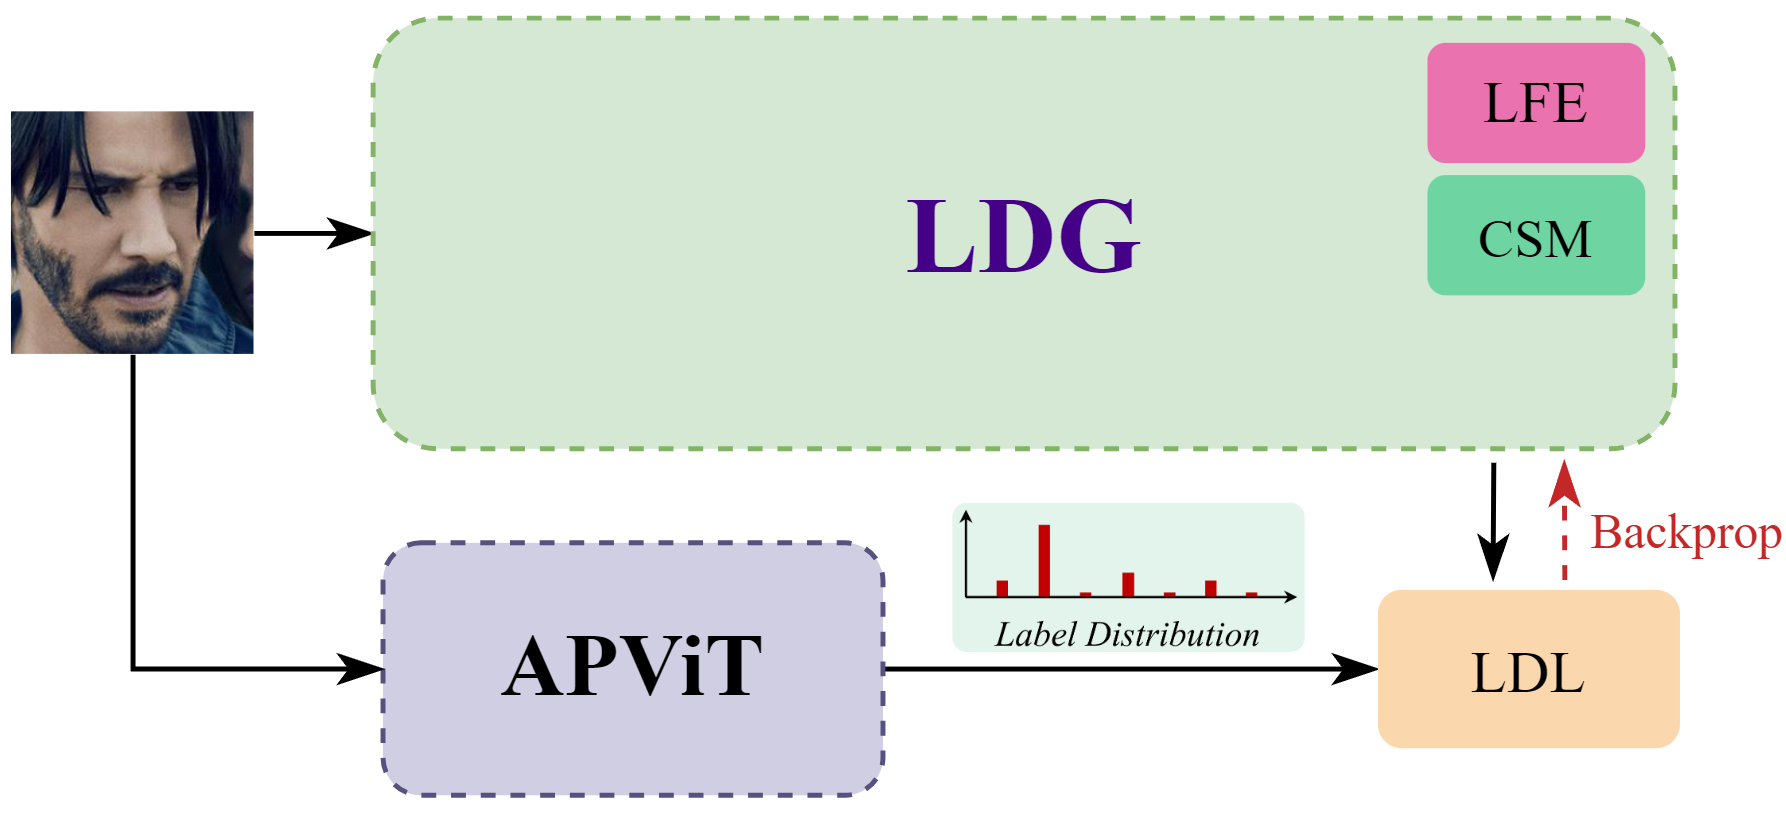
\includegraphics[width=1\columnwidth]{../images/chap_design/Phase 1 diagram.png}
		\caption[Phase I training pipeline]{Training pipeline for the first phase of the proposed algorithm. The IR-50 \cite{deng2019ir50} network is loaded with the backbone weights of APViT \cite{apvit2023} and enhanced with the local-global feature extraction modules from EfficientFace \cite{eff-face2021}. It is then trained using APViT as the distribution generator.}
		\label{fig:phase1-diagram}
	\end{center}
\end{figure}


The modified LDG is based on the same ResNet-50 architecture that serves as the feature extraction backbone of APViT. Three key modifications are proposed to enhance the LDG's FER performance and in turn the performance of the resulting EfficientFace variant. The design for this stage is depicted in figure \ref{fig:phase1-diagram}.

\textbf{1. FER-pretrained backbone weights from APViT:} Instead of initializing the ResNet-50 backbone with ImageNet \cite{deng2009imagenet} pretrained weights (as in the original EfficientFace approach), we initialize it with the backbone weights from a fully trained APViT model. Since APViT uses a hybrid architecture that includes convolutional layers before the transformer encoder, these pretrained weights are already specialized for facial expression recognition. This initialization provides the LDG with feature extractors that are tuned to capture expression-relevant patterns.

\textbf{2. Local-Global feature extraction modules:} We integrate the specialized local-global feature extraction modules from EfficientFace into the modified LDG architecture. These modules are inserted between the convolutional stages of the ResNet-50 backbone, allowing the network to extract both local facial features (such as subtle changes in specific facial regions) and global contextual information (such as overall facial configuration). This architectural enhancement helps the LDG generate more informative label distributions that capture the multi-scale nature of facial expressions.

\textbf{3. Knowledge distillation from APViT:} The modified LDG is trained using knowledge distillation, where the training objective is to minimize the difference between the LDG's output probability distributions and those generated by the fully trained APViT model. Specifically, we employ the same label distribution learning loss from EfficientFace to measure the discrepancy between the two distributions. This training procedure enables the modified LDG to learn to produce soft labels that approximate APViT's predictions while maintaining a more efficient architecture.

\subsubsection{Training EfficientFace with the Modified LDG}

Once the modified LDG is trained, it serves as the label distribution generator for training EfficientFace. The training procedure follows the original label distribution learning approach \cite{eff-face2021}, but with the modified LDG replacing the original ResNet-50 LDG.\\

During EfficientFace training, the modified LDG remains frozen and is used to generate soft label distributions for each training image. EfficientFace is then trained to minimize the loss between its predicted distributions and these soft labels. This two-stage knowledge transfer process, first from APViT to the modified LDG, then from the modified LDG to EfficientFace, should enable the lightweight model to benefit from APViT's superior representational capacity without the computational burden of using APViT directly during training. The design for this stage is depicted in figure \ref{fig:phase2-diagram}.\\

We employ a slightly tweaked version of the EfficientFace source code that fixes some minor bugs and limitations of the original implementation. The modified codebase is publicly available at \url{https://github.com/DavidCrgh/EfficientFace}.


\begin{figure}
	\begin{center}
		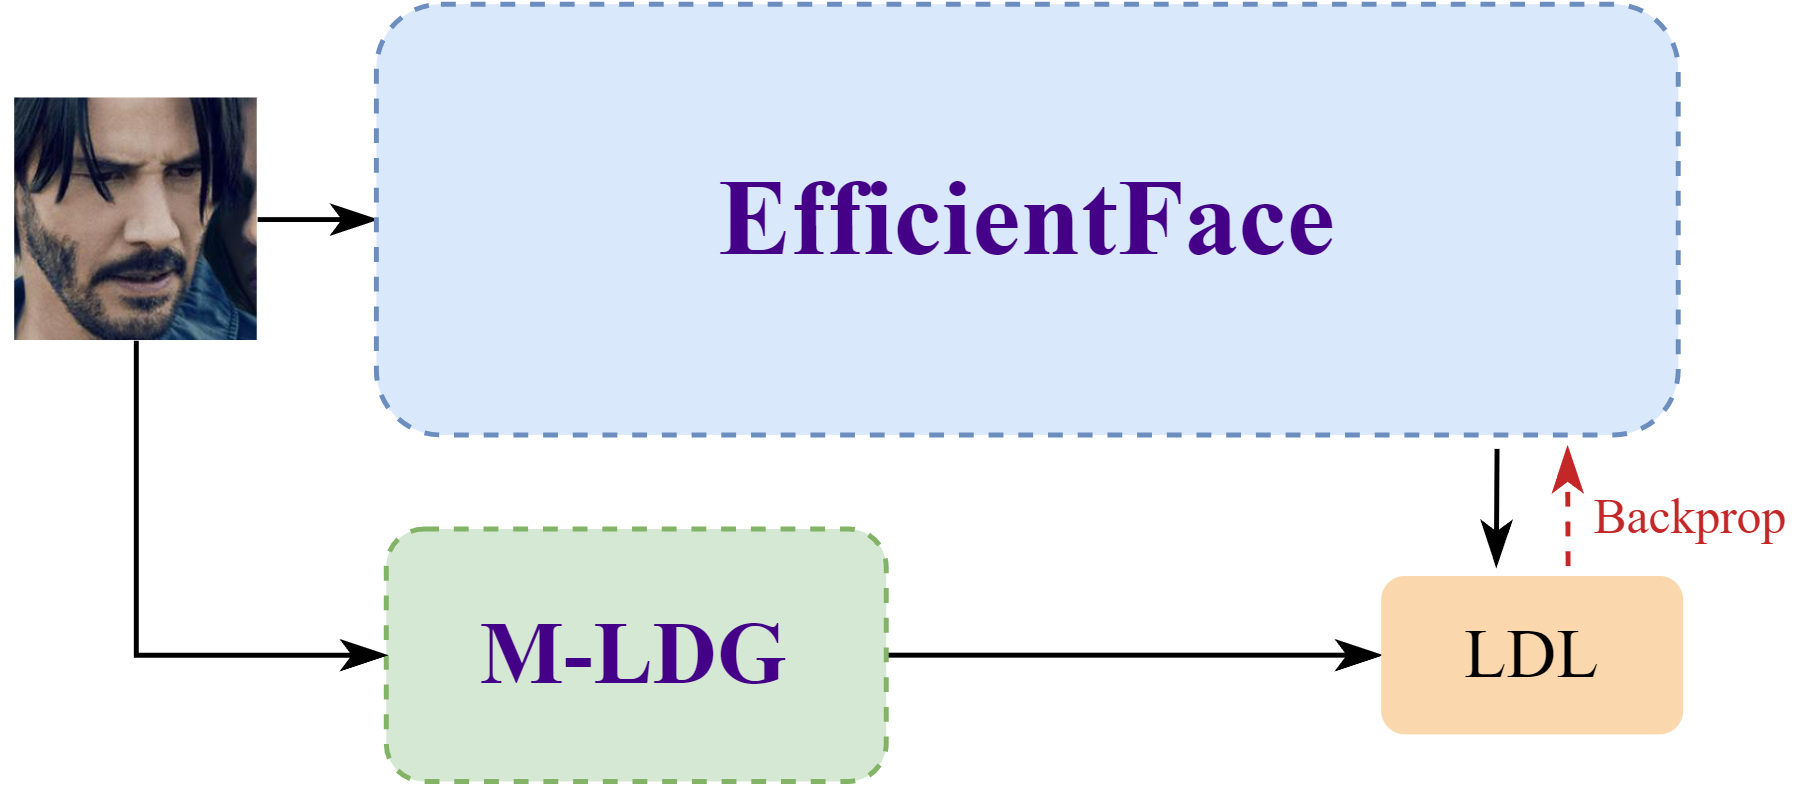
\includegraphics[width=1\columnwidth]{../images/chap_design/Phase 2 diagram.png}
		\caption[Phase II training pipeline]{Training pipeline for the second phase of the proposed algorithm. The modified LDG is used to train EfficientFace on the AffectNet dataset.}
		\label{fig:phase2-diagram}
	\end{center}
\end{figure}

\subsection{Dataset preprocessing}
Dataset preprocessing involves standardizing and transforming the facial images to create model-ready inputs. For each image, the pipeline first detects and aligns faces using RetinaFace \cite{retinaface2020} to account for pose variation and ensure facial landmarks are centered and consistently oriented. Images are then resized and padded to a fixed size of 112 x 112 pixels. These transformations ensure that all images fed to the models are properly aligned, uniformly sized, and consistently formatted, which is critical for robust model training. These steps are carried out once outside the training pipeline.\\

Additional preprocessing steps are applied at training and validation time. These steps follow the exact same procedure as the original EfficientFace architecture. For training, images are first randomly resized and cropped to the target size, followed by random horizontal flipping for data augmentation. Each image is then normalized using mean and standard deviation values matching the ImageNet dataset (mean=[0.485, 0.456, 0.406]; std=[0.229, 0.224, 0.225]). For validation and testing, images are simply resized to the target size, and normalized in the same way, but no random augmentation is applied.

\subsubsection{Image upscaling} \label{section:design-upsampling}
An important implementation detail is that the APViT and modified LDG architectures expect and are trained on 112 x 112 pixel images as input, while EfficientFace expects 224 x 224 sized images. To address this, we upscale the images to 224 x 224 during training in the second phase of the proposed algorithm. The upscaling is carried out using bilinear interpolation.

\subsection{Hyperparameter optimization}

Both phases of the experimental design follow the same general procedure. First, the experiment is executed across all factor combinations. From these runs, the best-performing combinations are selected and subjected to hyperparameter optimization. The optimization searches over learning rate, momentum, weight decay, and the learning rate schedule (adjustment frequency and reduction factor), using a Bayesian search with early termination (Hyperband \cite{hyperband2018}) to select the best configuration. The resulting optimized model is taken as the winner or representative of that phase. Phase II uses the Phase I winner whenever the modified LDG is the selected guidance network: the best modified LDG from Phase I is loaded as the frozen label distribution generator for training EfficientFace in the corresponding Phase II condition.

\subsection{Training APViT on AffectNet}\label{section:design-apvit-training}

As noted in the Requirements section, pretrained APViT weights for AffectNet were not publicly available at the time of this work. The network was therefore trained from scratch following the procedure described in the original APViT paper \cite{apvit2023}.\\

The public APViT codebase is oriented toward training on the RAF-DB dataset, so modifications were necessary to support training on AffectNet. These adaptations include changes to the data loading pipeline, class configuration, and evaluation scripts. The modified codebase is publicly available at \url{https://github.com/DavidCrgh/APViT}.\\

Table~\ref{tab:design-apvit-hyperparams} lists the key training hyperparameters used for this run. These values were taken directly from the configuration file provided in the original repository and kept unchanged.\\

\begin{table}[h]
    \centering
    \caption[APViT training hyperparameters for AffectNet]{APViT training hyperparameters used for training on AffectNet.}
    \label{tab:design-apvit-hyperparams}
    \begin{tabular}{ll}
        \toprule
        \textbf{Hyperparameter} & \textbf{Value} \\
        \midrule
		Training iterations (batches) & 6000 \\
        Input image size       & 112$\times$112 px \\
        Batch size             & 128 \\
        Optimizer              & SGD \\
        Learning rate          & $5 \times 10^{-4}$ \\
        Momentum               & 0.9 \\
        Weight decay           & $5 \times 10^{-4}$ \\
        LR schedule            & Cosine Annealing \\
        Gradient clip max norm & 10.0 \\
        ViT depth              & 8 layers \\
        ViT embedding dim      & 768 \\
        Attention heads        & 8 \\
        CNN pool (patches retained) & 160 \\
        \bottomrule
    \end{tabular}
\end{table}

The trained APViT achieved 64.2\% accuracy on AffectNet-7 and 57.31\% on AffectNet-8. These results are below the 66.91\% reported in the original paper \cite{apvit2023}, which was obtained on the same AffectNet-7 split, suggesting there is room for further tuning. Nevertheless, the trained model provides a functional teacher network for the proposed knowledge distillation pipeline.

\subsection{Limitations and Requirements}

This section outlines the key limitations and requirements of our proposed design, derived from the scope and limitations defined for this research project.

\subsubsection{Limitations}

Refer to section \ref{section:scope-limitations} for the limitations of this research project.

\subsubsection{Requirements}

\textbf{Pretrained models:} \label{section:design-pretrained-models} The proposed approach requires access to model weights for the APViT network pretrained on the AffectNet dataset. To the best of our knowledge, these weights are not publicly available. As such, we retrained the network from scratch using the same procedure as described in the original APViT paper \cite{apvit2023}.

\textbf{Computational resources:} The main computational resource required for executing the proposed approach is the available GPU memory. Phase I of the design requires more memory since it leverages the two heaviest networks: APViT and the modified LDG. In executions of Phase I, we noticed a memory requirement of approximately 16GB of VRAM per training run.

\textbf{Dataset access:} The execution of the proposed approach requires access to the 7-class and 8-class subsets of the AffectNet dataset \cite{affnet2019}.

\textbf{Software environment:} Execution of the training scripts requires an environment with the following software:
\begin{itemize}
    \item Python 3.10
    \item PyTorch 1.11 and CUDA 11.8
    \item MMCV 1.7.1
    \item WandB
    \item RetinaFace \cite{retinaface2020}
    \item A copy of the main code repository. (See \ref{section:implementation}).
\end{itemize}

\textbf{Face alignment tools:} The main code repository contains a script for face alignment using RetinaFace. Any of its dependencies must be installed in the execution environment.

\subsection{Implementation}\label{section:implementation}

The main code repository is hosted on GitHub and can be accessed at the following URL: \url{https://github.com/DavidCrgh/FER-MLDG}. The \texttt{src/networks} directory contains the implementations of the APViT, LDG, and EfficientFace architectures. Dataset preprocessing code, including face alignment with RetinaFace and conversion to the formats required by each network, is located in the \texttt{src/preproc} directory. Experiment execution is organized through Jupyter notebooks. The notebooks handle environment setup, configuration loading, and invocation of the underlying training scripts. Notebooks are also provided for executing the hyperparameter optimization process using WandB Sweeps.
% Results
\chapter{Results}
\epigraph{``Another quote.''}{\vspace{10pt}Another author}
\label{chapter:results}
\newpage

This chapter reports the findings of the two experimental phases described in chapters \nameref{chapter:methodology} and \nameref{chapter:design}. The response variable for both phases is top-1 validation accuracy on the AffectNet dataset \cite{affnet2019}. We present factorial results, main effect estimates, learning curve observations, hyperparameter optimization outcomes, and statistical test results in the order they were produced. Interpretation and analysis of these findings are deferred to the \nameref{chapter:discussion} chapter.\\

\section{Phase I: label distribution generator ablation}
\label{section:results-phase1}

\subsection{Factorial results}
\label{section:results-phase1-factorial}

The Phase I full $2^4$ factorial design yielded 16 experimental runs covering all combinations of the four factors defined in Table~\ref{tab:p1-factors}: pretrained backbone weights (A), local-global feature extraction modules (B), APViT guidance (C), and dataset (D). The treatment combinations are enumerated in Table~\ref{tab:p1-runs}. Table \ref{tab:results-p1-ranked} presents all 16 runs ranked by best validation accuracy.\\

\begin{table}[h!]
    \centering
    \begin{tabular}{@{}rrccccrr@{}}
    \toprule
    \textbf{Rank} & \textbf{Treat.} & \textbf{A} & \textbf{B} & \textbf{C} & \textbf{D} & \textbf{Best Acc.\ (\%)} & \textbf{Best Ep.} \\
    \midrule
    1  & 12 & $-$ & $-$ & $+$ & AN-7 & 63.31 & 17 \\
    2  &  0 & $+$ & $+$ & $+$ & AN-7 & 63.29 & 15 \\
    3  &  4 & $+$ & $-$ & $+$ & AN-7 & 63.20 & 13 \\
    4  &  8 & $-$ & $+$ & $+$ & AN-7 & 63.14 & 27 \\
    5  &  1 & $+$ & $+$ & $+$ & AN-8 & 57.06 & 14 \\
    6  &  5 & $+$ & $-$ & $+$ & AN-8 & 56.99 & 18 \\
    7  &  9 & $-$ & $+$ & $+$ & AN-8 & 56.84 & 29 \\
    8  & 13 & $-$ & $-$ & $+$ & AN-8 & 56.76 & 27 \\
    9  &  2 & $+$ & $+$ & $-$ & AN-7 & 55.51 & 23 \\
    10 & 14 & $-$ & $-$ & $-$ & AN-7 & 55.34 & 27 \\
    11 &  6 & $+$ & $-$ & $-$ & AN-7 & 55.26 & 28 \\
    12 & 10 & $-$ & $+$ & $-$ & AN-7 & 55.17 & 27 \\
    13 & 11 & $-$ & $+$ & $-$ & AN-8 & 49.24 & 24 \\
    14 &  7 & $+$ & $-$ & $-$ & AN-8 & 49.24 & 24 \\
    15 &  3 & $+$ & $+$ & $-$ & AN-8 & 49.01 & 29 \\
    16 & 15 & $-$ & $-$ & $-$ & AN-8 & 48.71 & 28 \\
    \bottomrule
    \end{tabular}
    \smallskip

    \footnotesize{AN-7 = AffectNet-7; AN-8 = AffectNet-8. $+$ / $-$ denote the high / low factor level. Treatment IDs correspond to the run numbering defined in Table~\ref{tab:p1-runs}.}
    \caption[Phase I factorial results ranked by accuracy]{All 16 treatment combinations of the Phase I $2^4$ factorial design, ranked by best validation accuracy. Factors are: A (pretrained backbone weights), B (local-global feature extraction modules), C (APViT guidance), D (dataset subset).}
    \label{tab:results-p1-ranked}
\end{table}

The 16 runs span a range from 63.31\% to 48.71\%, with a mean of 56.13\% and an overall standard deviation of 5.05\%. The eight runs with APViT guidance enabled (C+) occupy ranks 1 through 8 and cluster between 56.76\% and 63.31\%, while the eight runs without guidance (C-) occupy ranks 9 through 16 and cluster between 48.71\% and 55.51\%. The highest accuracy (63.31\%) was achieved by treatment 12 (C+, A-, B-, AffectNet-7) and the lowest (48.71\%) by treatment 15 (C-, A-, B-, AffectNet-8). Within each C level, runs trained on AffectNet-7 consistently outperformed their AffectNet-8 counterparts by approximately 6 percentage points, confirming the dominant roles of factors C and D before formal effect estimation.\\

\subsection{Main effects and interactions}
\label{section:results-phase1-effects}

Main effect estimates were computed using Yates's algorithm \cite{montgomery2017design}. The results are summarized in Table \ref{tab:results-p1-effects} and visualized in figure \ref{fig:results-p1-halfnormal}.\\

\begin{table}[h!]
    \centering
    \begin{tabular}{@{}lrr@{}}
    \toprule
    \textbf{Factor / Interaction} & \textbf{Effect} & \textbf{Abs(Effect)} \\
    \midrule
    C (APViT guidance)         & $+7.889$ & 7.889 \\
    D (Dataset)                & $-6.297$ & 6.297 \\
    A (Pretrained backbone)    & $+0.129$ & 0.129 \\
    A$\times$D                 & $-0.058$ & 0.058 \\
    B$\times$D                 & $-0.056$ & 0.056 \\
    B (GL modules)             & $+0.056$ & 0.056 \\
    B$\times$C                 & $-0.040$ & 0.040 \\
    C$\times$D                 & $+0.025$ & 0.025 \\
    A$\times$C                 & $-0.010$ & 0.010 \\
    A$\times$B                 & $-0.008$ & 0.008 \\
    Higher-order ($\geq$ 3 factor) & \multicolumn{1}{c}{---} & $< 0.18$ \\
    \bottomrule
    \end{tabular}
    \caption[Phase I effect estimates (Yates's algorithm)]{Main effect and interaction estimates for the Phase I $2^4$ factorial design computed with Yates's algorithm. Values are in percentage points (pp). Effects are listed in decreasing order of absolute value.}
    \label{tab:results-p1-effects}
\end{table}

\begin{figure}[h!]
    \centering
    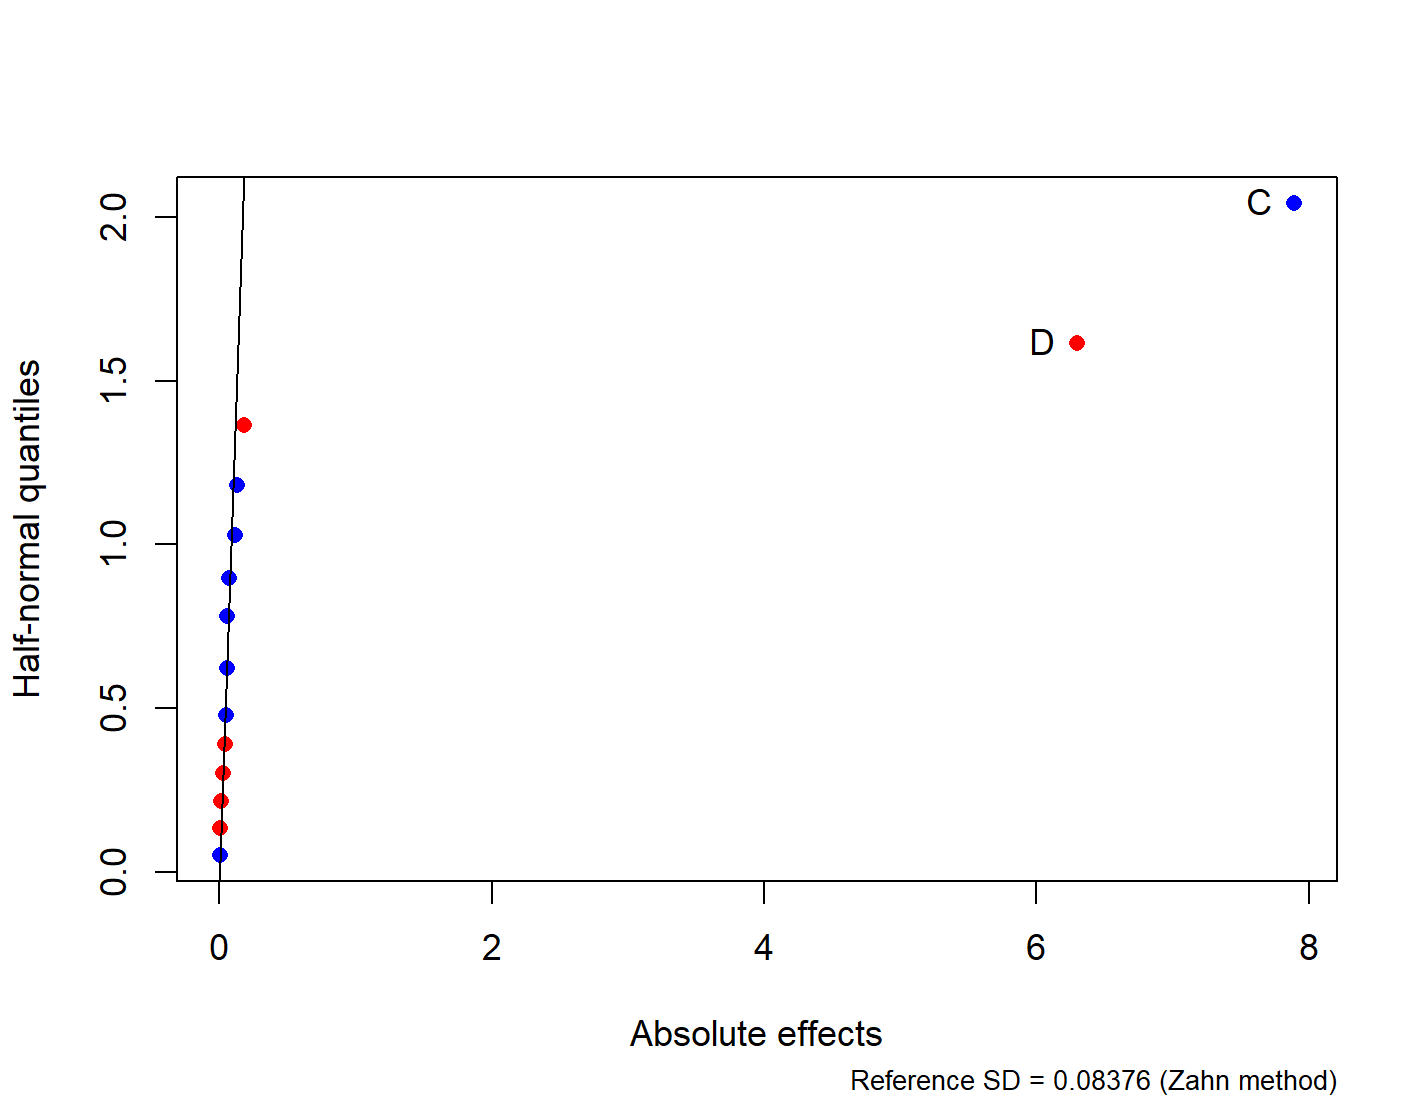
\includegraphics[width=0.7\columnwidth]{../images/chap_results/halfnormal.png}
    \caption[Phase I half-normal effects plot]{Half-normal probability plot of the Phase I effect estimates from Yates's algorithm. Effects that deviate substantially from the reference line are considered active \cite{montgomery2017design}. Only active effects are labeled.}
    \label{fig:results-p1-halfnormal}
\end{figure}

Factor C (APViT guidance) produced the largest main effect at +7.889 percentage points (pp), followed by factor D (dataset) at -6.297 pp, indicating that the AffectNet-7 subset yields higher accuracy than AffectNet-8. Factors A (pretrained backbone weights) and B (local-global feature extraction modules) showed negligible effects of +0.129 pp and +0.056 pp, respectively. All interaction effects were also negligible: the C×D interaction was +0.025 pp, and all remaining two-factor and higher-order interactions fell below 0.18 pp in absolute value. The within-cell standard deviations, obtained after pooling A and B, ranged from 0.08\% to 0.25\%, confirming that A and B contribute no meaningful variance to the response.\\

The C×D interaction quantifies whether the benefit of APViT guidance varies across datasets. The near-zero interaction estimate of +0.025 pp indicates that the contributions of C and D are negligible. Figure \ref{fig:results-p1-interaction} shows the interaction line plot for C and D after pooling A and B.\\

\begin{figure}[h!]
    \centering
    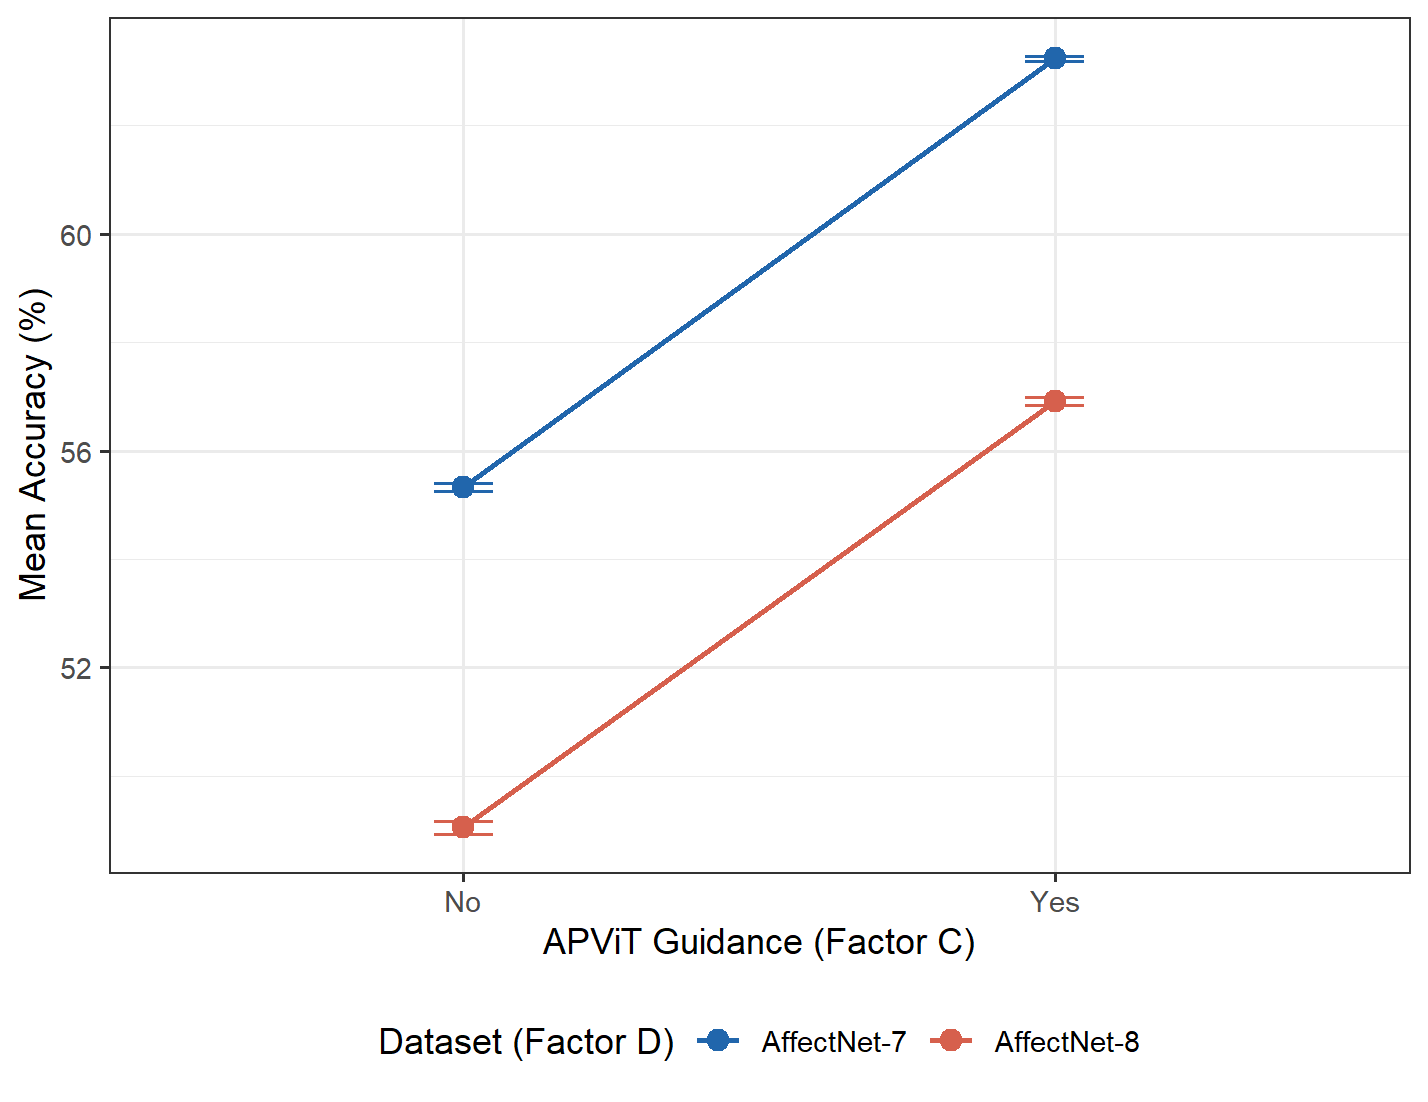
\includegraphics[width=0.7\columnwidth]{../images/chap_results/cxd_interaction.png}
    \caption[Phase I C×D interaction plot]{Interaction plot for factors C (APViT guidance) and D (dataset) after pooling negligible factors A and B. The near-parallel lines confirm the negligible C×D interaction (+0.025 pp).}
    \label{fig:results-p1-interaction}
\end{figure}

\subsection{Learning behavior}
\label{section:results-phase1-curves}

Training and validation accuracy curves were recorded for all 16 Phase I runs via WandB. Figure \ref{fig:results-p1-curves} presents representative curves for the four C×D conditions.\\

\begin{figure}[h!]
    \centering
    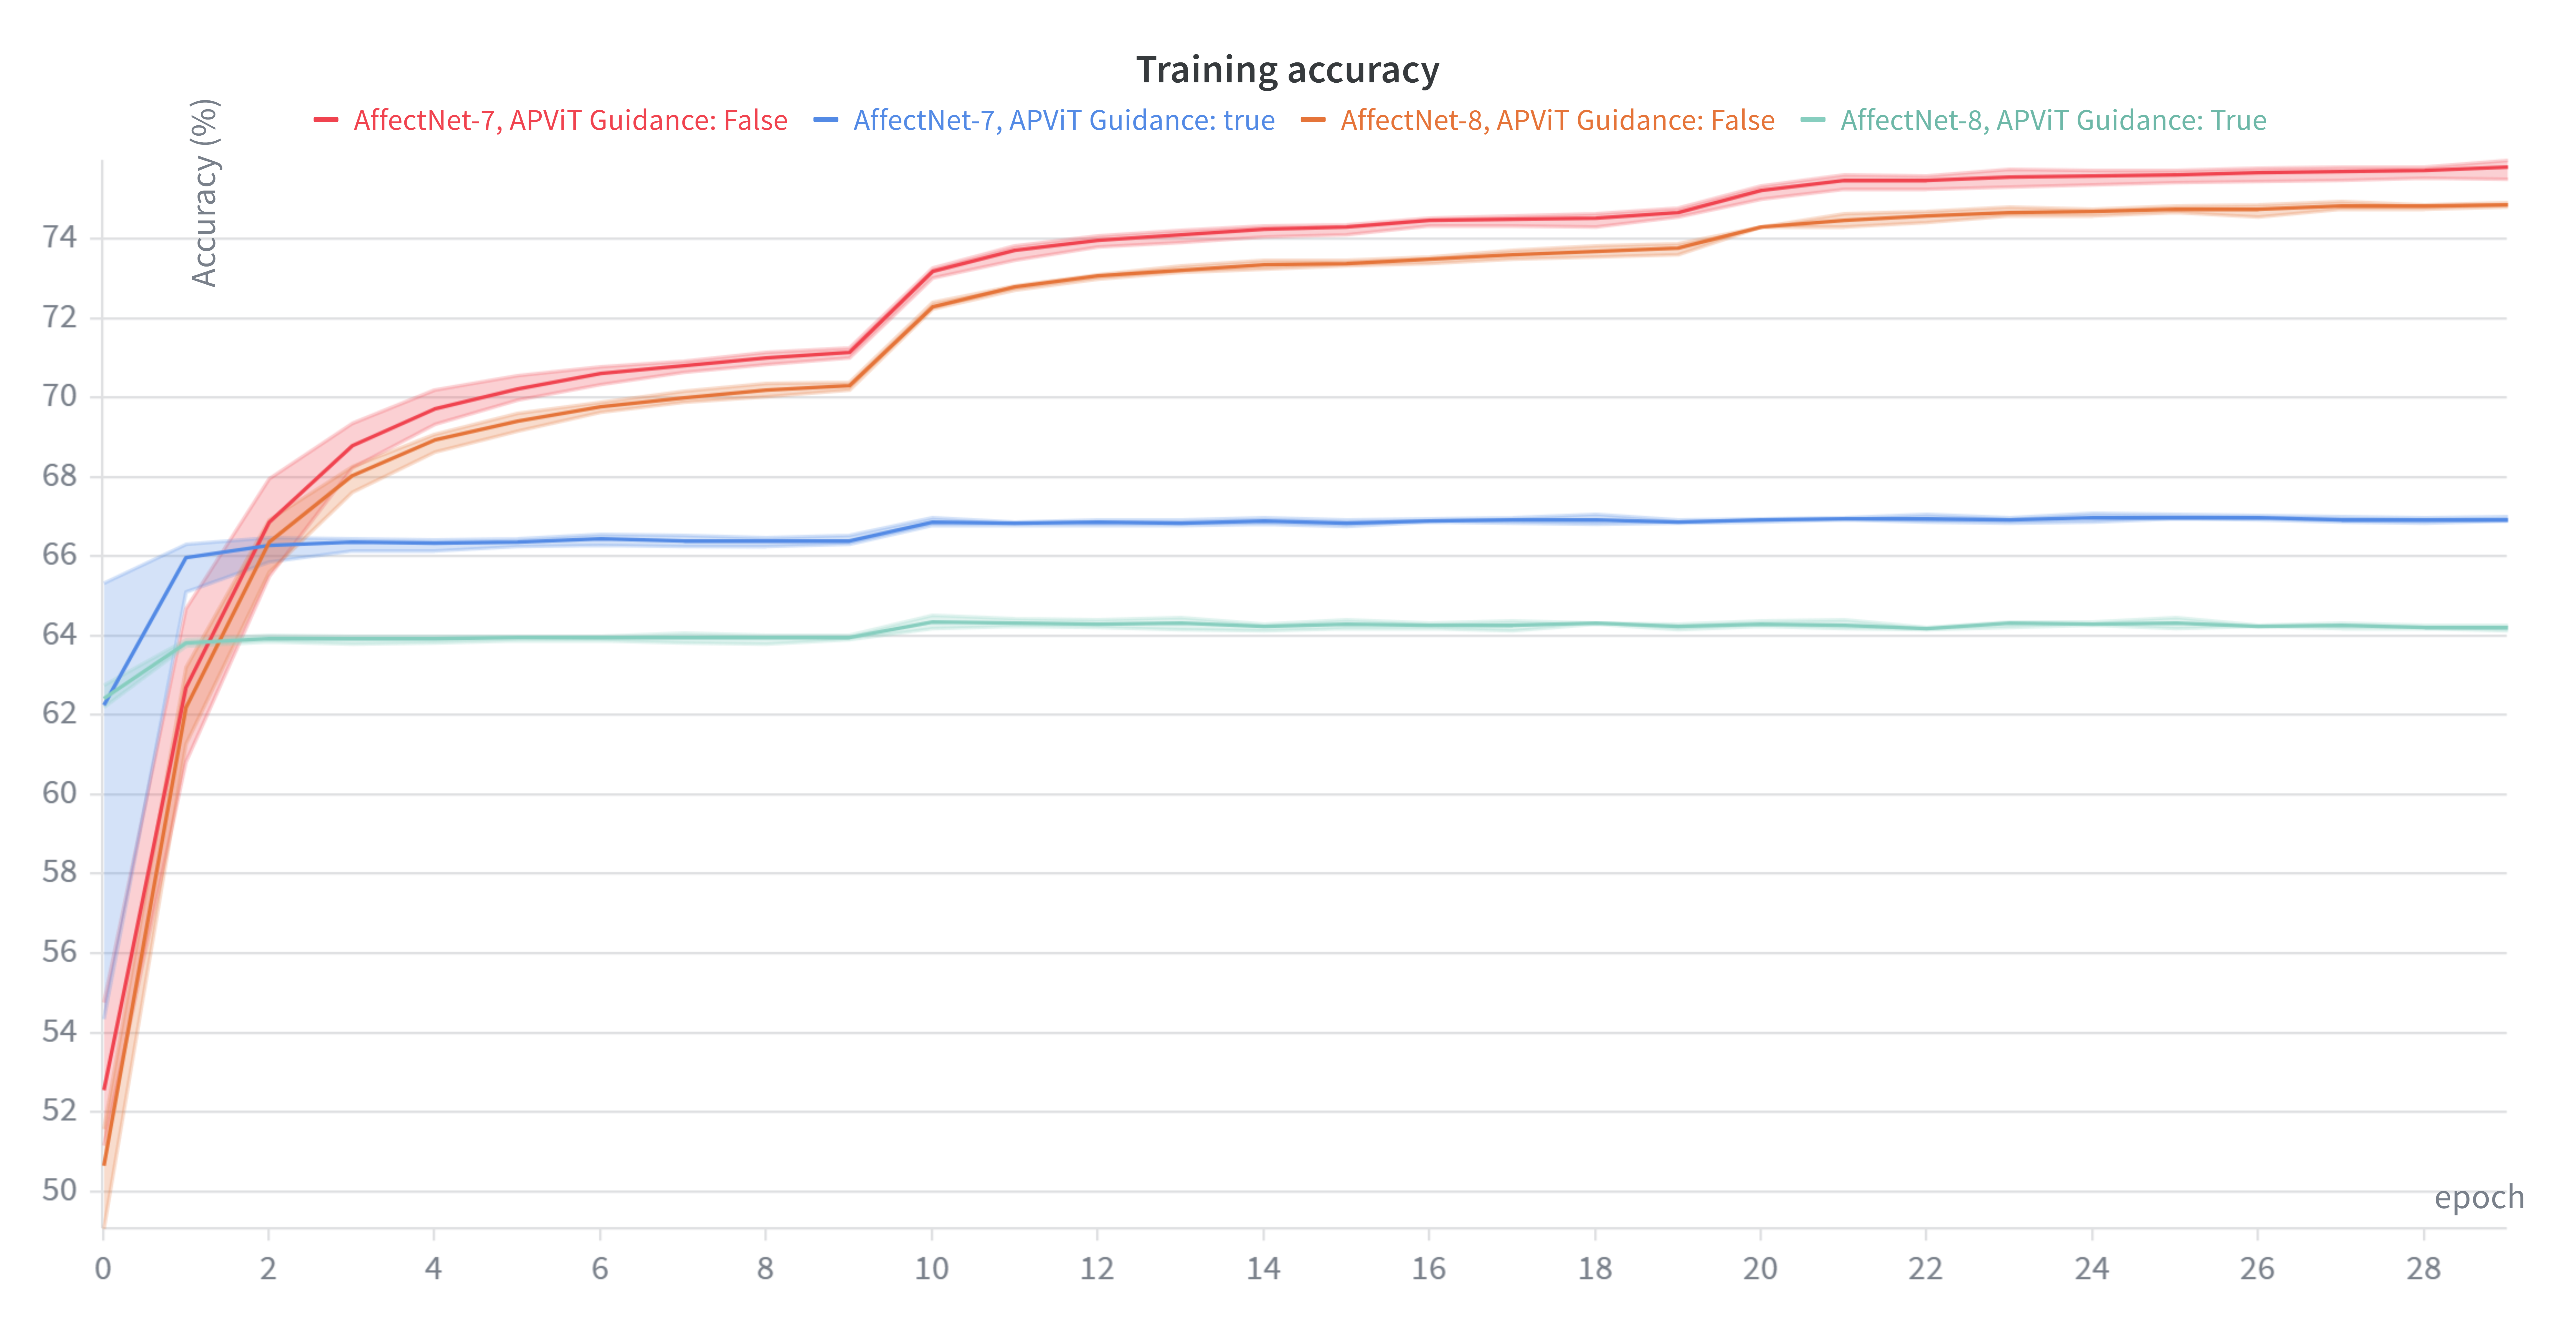
\includegraphics[width=1\columnwidth]{../images/chap_results/trainingcurve.png}
    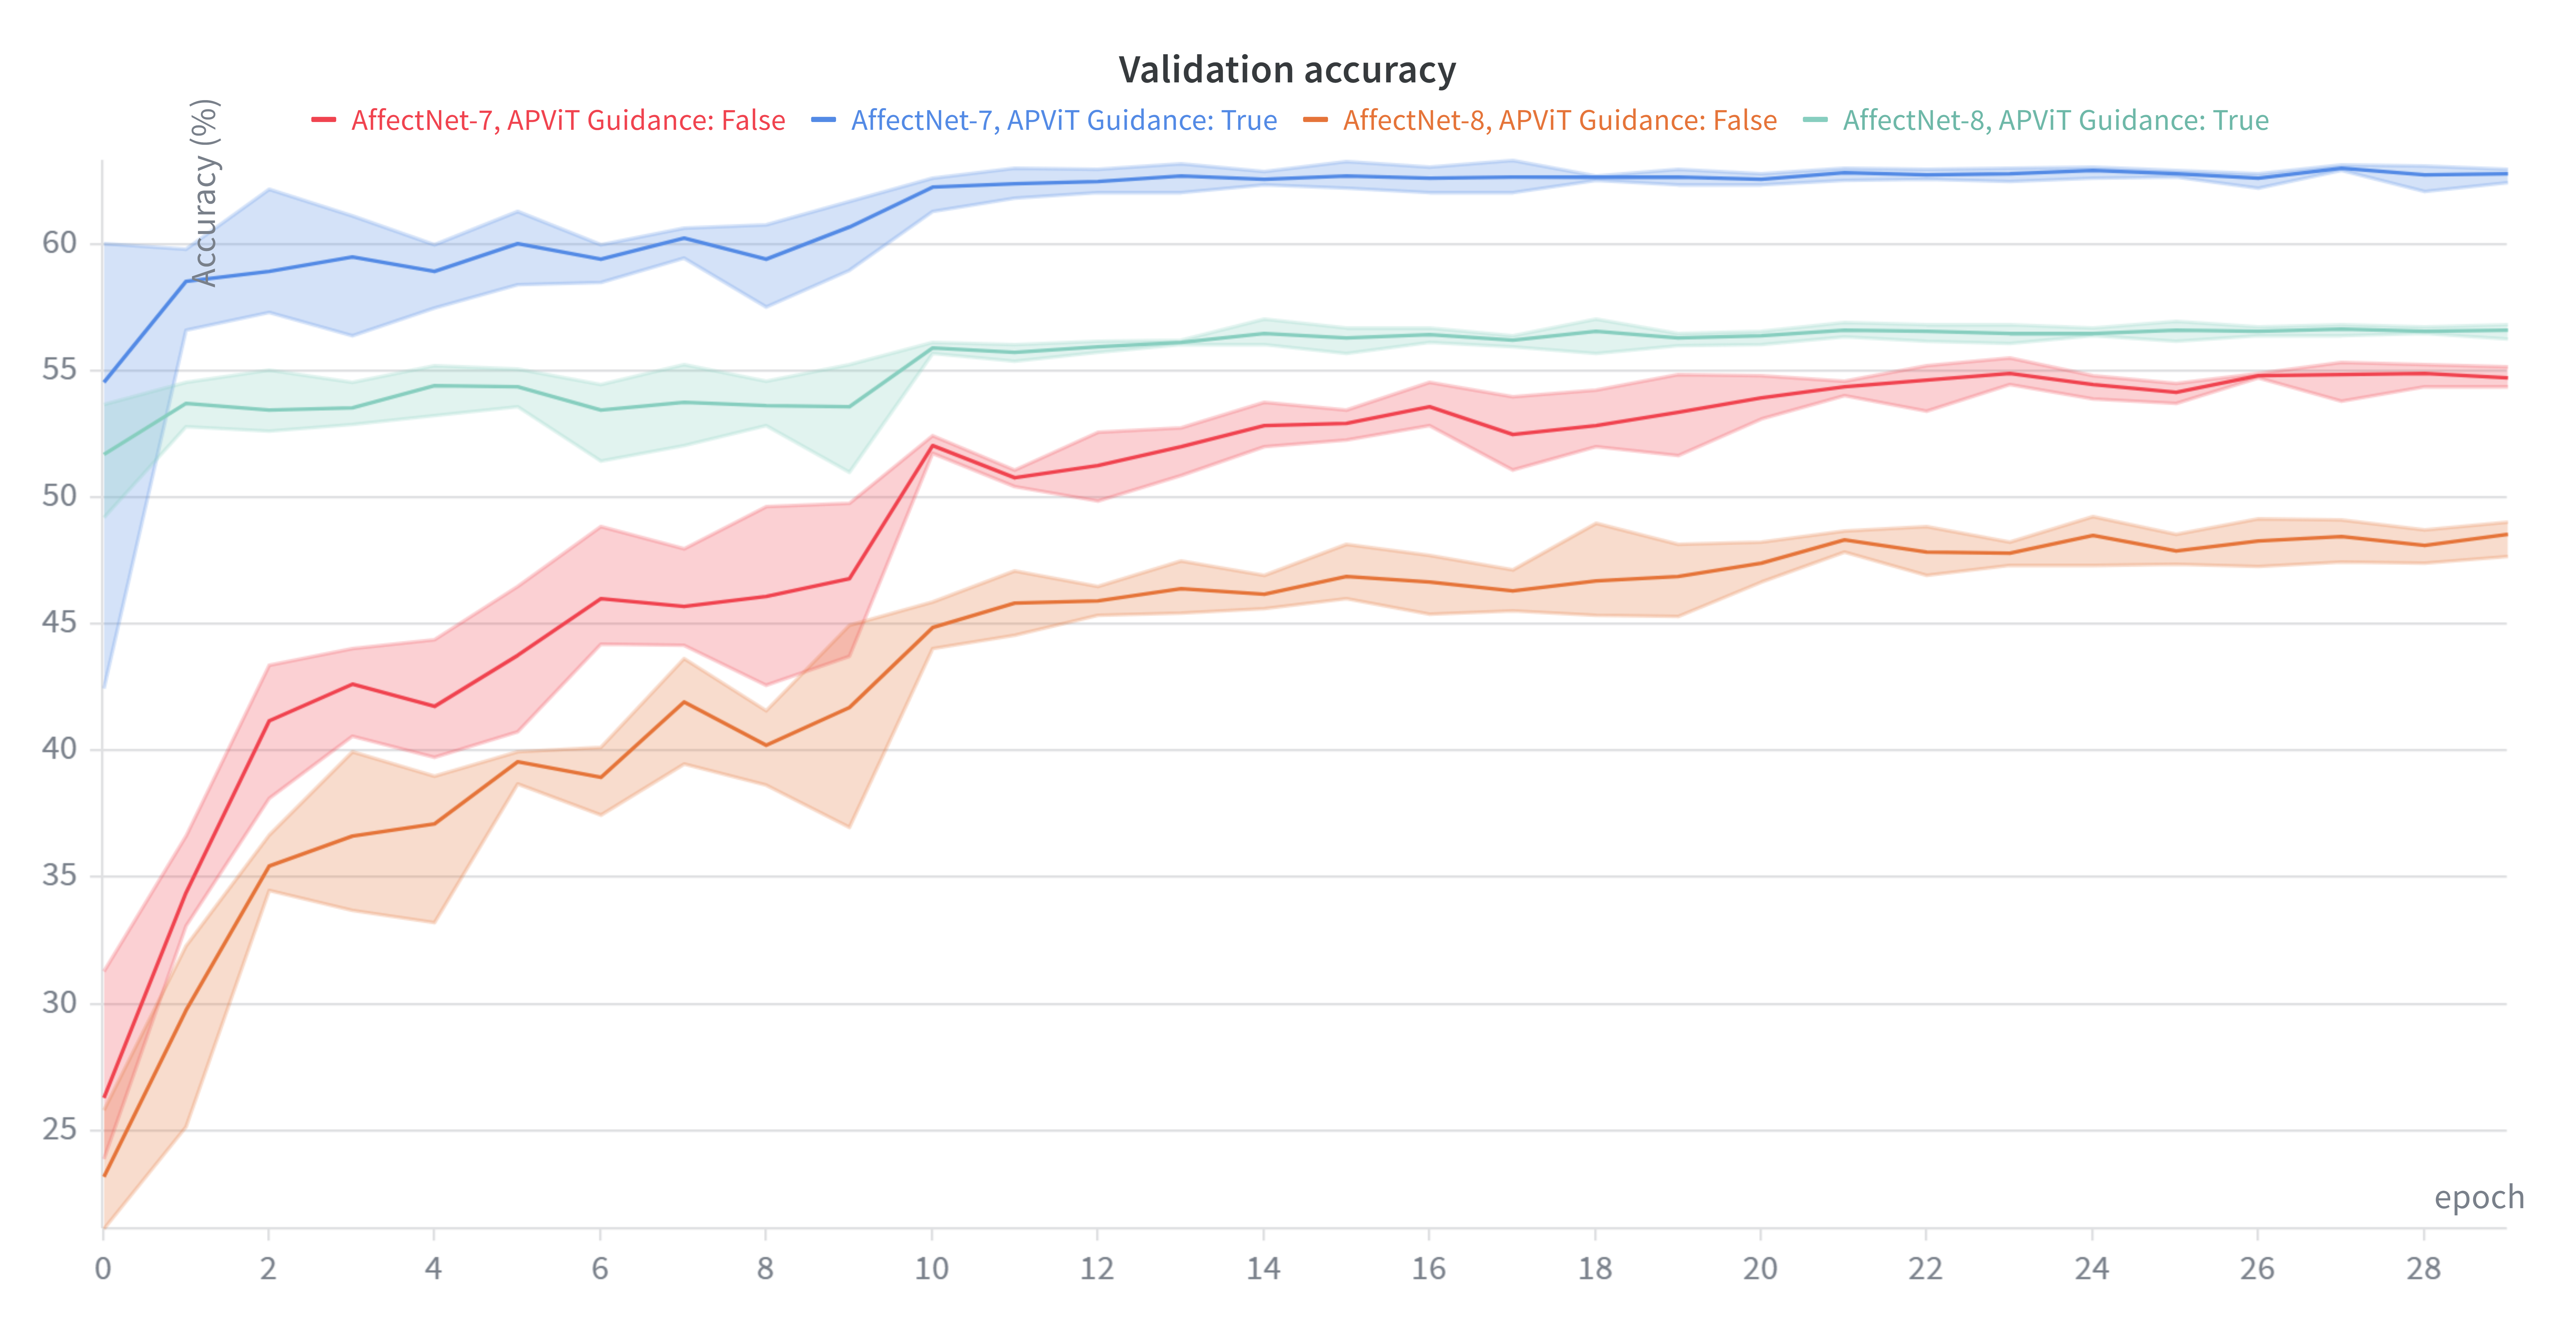
\includegraphics[width=1\columnwidth]{../images/chap_results/validationcurve.png}
    \caption[Phase I training curves by C×D condition]{Representative training and validation accuracy curves for the four C×D conditions in Phase I. Each curve aggregates runs (mean) within the same C×D cell across varying A and B levels.}
    \label{fig:results-p1-curves}
\end{figure}

We observe two distinct training behaviors depending on the state of factor C. Runs with APViT guidance (C+) converged to their best validation accuracy between epochs 13 and 27, with a mean train-validation gap of approximately 5-7\%. Runs without APViT guidance (C-) exhibited severe overfitting, with training accuracy reaching 75-76\% while validation accuracy plateaued early, yielding a mean train-validation gap of approximately 24\%. The learning rate schedule, which applies a decay factor at epochs 10 and 20, produced visible accuracy steps in C- runs that are attenuated or absent in C+ runs. Across all conditions, runs trained on AffectNet-8 plateaued approximately 6 pp below their AffectNet-7 counterparts.\\

\subsection{Hyperparameter optimization and the M-LDG}
\label{section:results-phase1-optim}

Following the factorial experiment, a Bayesian hyperparameter search using WandB Sweeps with Hyperband early termination \cite{hyperband2018} was applied to the two best-performing factor combinations for each dataset (0, 1, 5, and 12). Eight 12-epoch trials were conducted across the two datasets, after which the best-identified configurations were confirmed with full 30-epoch runs. Table \ref{tab:results-p1-sweep} reports all eight sweep trials.\\

\begin{table}[h!]
    \centering
    \begin{tabular}{@{}rllllllr@{}}
    \toprule
    \textbf{\#} & \textbf{Dataset} & \textbf{LR} & \textbf{M} & \textbf{WD} & \textbf{F} & \textbf{Freq.} & \textbf{Best Acc.\ (\%)} \\
    \midrule
    1 & AN-7 & 0.00205 & 0.865 & $5.08\times10^{-3}$ & 0.561 & 12 & \textbf{64.77} \\
    2 & AN-7 & 0.00205 & 0.944 & $1.35\times10^{-6}$ & 0.193 & 10 & 63.97 \\
    3 & AN-7 & 0.01461 & 0.861 & $2.50\times10^{-6}$ & 0.138 & 10 & 63.89 \\
    4 & AN-7 & 0.04980 & 0.888 & $8.01\times10^{-6}$ & 0.338 &  5 & 63.46 \\
    5 & AN-7 & 0.02782 & 0.931 & $1.76\times10^{-5}$ & 0.600 &  8 & 63.20 \\
    \midrule
    6 & AN-8 & 0.01856 & 0.932 & $1.16\times10^{-6}$ & 0.474 &  3 & \textbf{57.49} \\
    7 & AN-8 & 0.02003 & 0.937 & $1.37\times10^{-6}$ & 0.516 &  3 & 57.29 \\
    8 & AN-8 & 0.00430 & 0.885 & $4.09\times10^{-6}$ & 0.543 & 12 & 57.21 \\
    \bottomrule
    \end{tabular}
    \caption[Phase I hyperparameter sweep results]{Hyperparameter configurations and best validation accuracies for the eight Phase I sweep trials. Accuracy values are from 12-epoch runs with Hyperband early termination. M = Momentum, WD = Weight Decay, F = Factor, Freq = Frequency.}
    \label{tab:results-p1-sweep}
\end{table}

The resulting optimized network, achieved 64.34\% on AffectNet-7 (best epoch: 9) and 57.71\% on AffectNet-8 (best epoch: 12) in their respective 30-epoch confirmatory runs. These results represent improvements of +1.03 pp and +0.65 pp over the best ablation runs with C=True (63.31\% and 57.06\%). This optimized variant is used as the singular M-LDG network in the next phase of this study. Table \ref{tab:results-p1-hyperparams} compares the default and optimized hyperparameter configurations used to train the M-LDG.\\

\begin{table}[h!]
    \centering
    \begin{tabular}{@{}lllll@{}}
    \toprule
    \textbf{Parameter} & \shortstack{\textbf{Default}\\\textbf{(Ablation)}} & \shortstack{\textbf{Optimized}\\\textbf{(AN-7)}} & \shortstack{\textbf{Optimized}\\\textbf{(AN-8)}} & \textbf{Change} \\
    \midrule
    Learning Rate  & 0.100                       & 0.024                     & 0.032                     & $\downarrow$ 3--4$\times$ lower \\
    Momentum       & 0.900                       & 0.860                     & 0.948                     & Dataset-specific \\
    Weight Decay   & $1.0\times10^{-4}$          & $8.8\times10^{-6}$        & $1.5\times10^{-6}$        & $\downarrow$ 10--70$\times$ lower \\
    LR Factor      & 0.100                       & 0.209                     & 0.450                     & $\uparrow$ Less aggressive \\
    Adjust Freq    & 10                          & 10                        & 3                         & Dataset-specific \\
    \bottomrule
    \end{tabular}
    \caption[Phase I default vs. optimized hyperparameters]{Default (ablation) and optimized hyperparameter configurations for the M-LDG on each AffectNet subset. Arrows indicate the direction of change relative to the default.}
    \label{tab:results-p1-hyperparams}
\end{table}

The optimized configurations differ from the defaults in three main respects: the learning rate is 3 to 4 times lower, the weight decay is 10 to 70 times lower, and the LR reduction factor is substantially less aggressive (0.209 for AffectNet-7 and 0.450 for AffectNet-8, compared to the default of 0.1). The AffectNet-7 M-LDG converged rapidly, reaching within 0.5 pp of its best accuracy by epoch 6, with a final train-validation gap of 2.71 pp. The AffectNet-8 M-LDG required more epochs to stabilize, with a final gap of 7.19 pp, reflecting the increased difficulty of the 8-class task.\\

\section{Statistical assumption tests}
\label{section:results-assumptions}

Prior to the two-way ANOVA, we verified the normality of residuals and the homogeneity of variance as required by the ANOVA assumptions. Both assumption tests were conducted on the Phase I data after pooling the negligible factors A and B into the error term, retaining C and D as the active factors.\\

The Shapiro-Wilk test for normality of residuals yielded $W = 0.9447$ ($p = 0.410$), providing no evidence against the normality assumption. Levene's test for homogeneity of variance produced $F(3, 12) = 1.317$ ($p = 0.314$), indicating no significant difference in variance across the four C×D cells. Both assumptions for parametric ANOVA are therefore satisfied. Figure \ref{fig:results-assumptions} shows the normal Q-Q plot of residuals and the residuals-versus-fitted plot used to assess these assumptions visually.\\

\begin{figure}[h!]
    \centering
    \begin{minipage}{0.49\columnwidth}
        \centering
        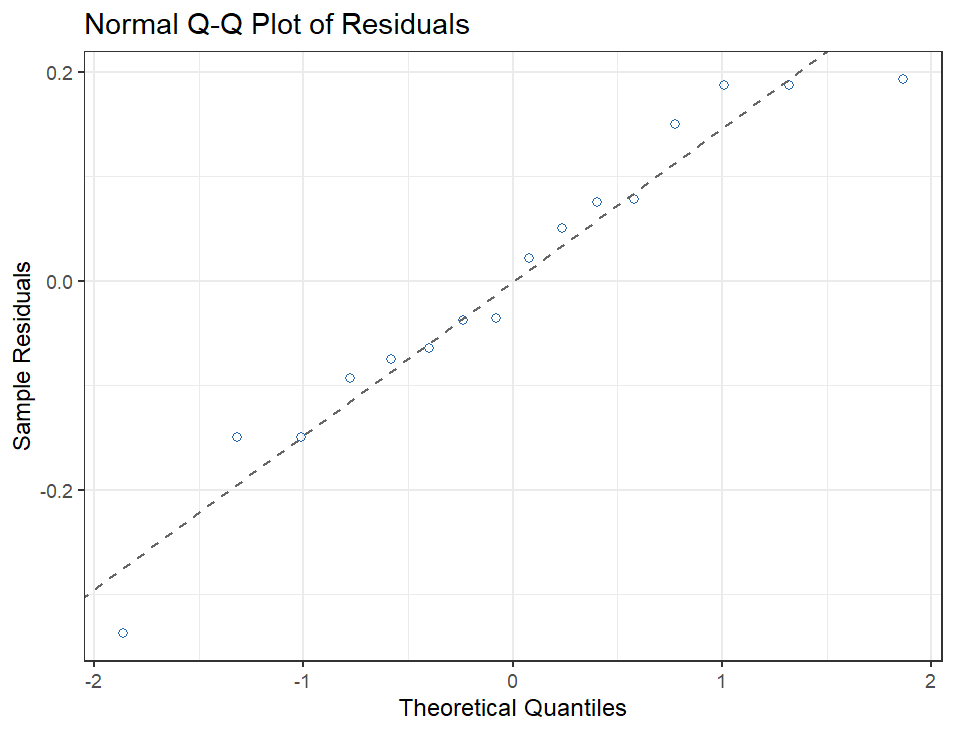
\includegraphics[width=\linewidth]{../images/chap_results/normalqq.png}
    \end{minipage}\hfill
    \begin{minipage}{0.49\columnwidth}
        \centering
        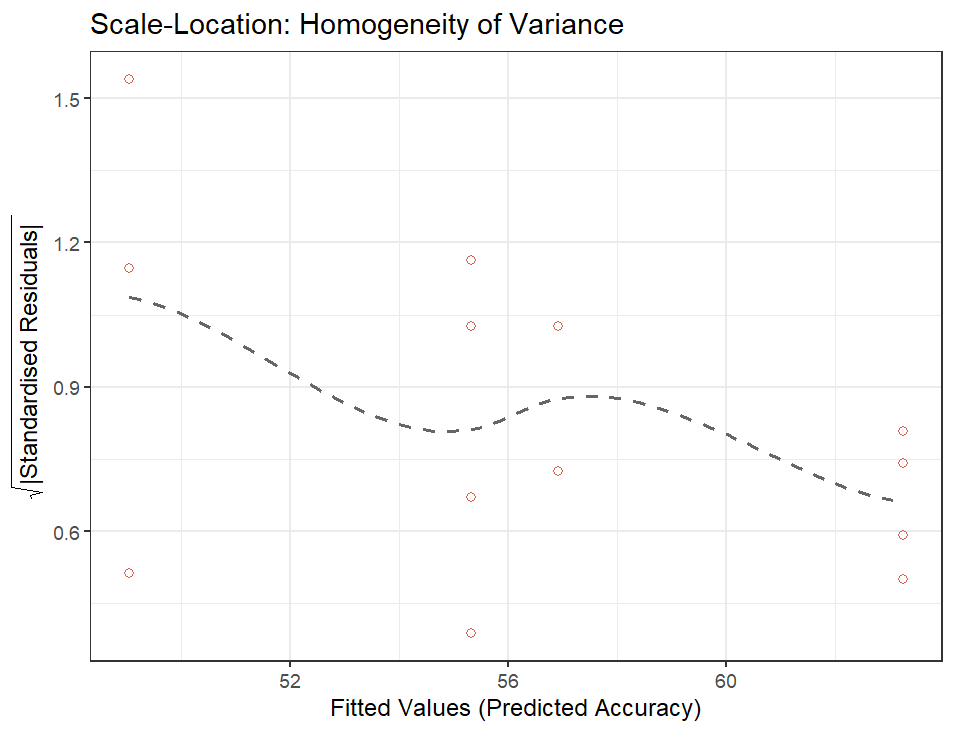
\includegraphics[width=\linewidth]{../images/chap_results/homovar.png}
    \end{minipage}
    \caption[Phase I ANOVA assumption plots]{Phase I ANOVA assumption checks after pooling factors A and B. Left: normal Q-Q plot of residuals; close alignment with the reference diagonal supports normality (Shapiro-Wilk $W = 0.9447$, $p = 0.410$). Right: residuals versus fitted values for the two-way ANOVA model; relatively constant spread suggests homoscedasticity, confirmed by Levene's test ($F(3, 12) = 1.317$, $p = 0.314$).}
    \label{fig:results-assumptions}
\end{figure}

\section{Two-way ANOVA results}
\label{section:results-anova}

A two-way ANOVA was performed on the Phase I data with best validation accuracy as the response and APViT guidance (C) and dataset (D) as the predictors, following the procedure defined in the \nameref{chapter:methodology} chapter. Given their low effect estimates, we pool together factors A and B to increase the reliability of the results. The criteria for pooling is based on visual analysis via the half-normal plot in Figure \ref{fig:results-p1-halfnormal}. Table \ref{tab:results-anova} presents the ANOVA table.\\

\begin{table}[h!]
    \centering
    \begin{tabular}{@{}lrrrrl@{}}
    \toprule
    \textbf{Source} & \textbf{df} & \textbf{SS} & \textbf{MS} & \textbf{F} & \textbf{$p$-value} \\
    \midrule
    APViT guidance (C)  & 1  & 248.97 & 248.97 & 9196.84 & $< 2\times10^{-16}$\,*** \\
    Dataset (D)         & 1  & 158.59 & 158.59 & 5858.17 & $< 2\times10^{-16}$\,*** \\
    C $\times$ D        & 1  &   0.002 &   0.002 &   0.092 & 0.767\phantom{$\times10^{-16}$\,***} \\
    Residuals           & 12 &   0.325 &   0.027 & & \\
    \bottomrule
    \end{tabular}
    \smallskip

    \footnotesize{Significance codes: *** $p < 0.001$. Factors A and B were pooled into the residuals.}
    \caption[Phase I two-way ANOVA]{Two-way ANOVA results for Phase I. Factors A and B were pooled into the residual after the effect estimation step; the model retains only factors C (APViT guidance) and D (dataset).}
    \label{tab:results-anova}
\end{table}

Both main effects were highly significant, while their interaction was not. APViT guidance (C) yielded $F(1, 12) = 9196.84$ ($p < 2 \times 10^{-16}$), the dataset (D) yielded $F(1, 12) = 5858.17$ ($p < 2 \times 10^{-16}$), and the C×D interaction was negligible ($F(1, 12) = 0.092$, $p = 0.767$). The residual term in Table \ref{tab:results-anova} is very small: repeated runs under the same condition landed within roughly 0.16 percentage points of one another, so the observed differences between conditions are highly reproducible rather than the product of random fluctuation.\\

To measure how much each factor matters in practice, we report effect sizes as eta-squared ($\eta^2$), the proportion of the total variation in accuracy explained by a factor. Dividing each factor's sum of squares in Table \ref{tab:results-anova} by the total sum of squares (407.89) gives $\eta^2 = 0.610$ for APViT guidance and $\eta^2 = 0.389$ for the dataset, with the interaction below 0.001. Together these two factors explain about 99.9\% of the systematic variation in accuracy. We therefore reject the null hypothesis that all treatment combinations yield the same mean accuracy: both APViT guidance and the choice of dataset produce statistically significant differences in performance.\\

\section{Phase II: EfficientFace guidance comparison}
\label{section:results-phase2}

\subsection{Cell means and replication}
\label{section:results-phase2-cells}

Phase II employed a $2^2$ factorial design with two replicates per treatment combination, as described in Table~\ref{tab:p2-runs}. The two factors were guidance network (G: M-LDG or APViT) and dataset (D: AffectNet-7 or AffectNet-8). A total of eight EfficientFace training runs were conducted, each for 45 epochs. Table \ref{tab:results-p2-cells} reports the individual run results and cell means.\\

\begin{table}[h!]
    \centering
    \begin{tabular}{@{}llrrrrl@{}}
    \toprule
    \textbf{Guidance (G)} & \textbf{Dataset (D)} & \textbf{Rep.\ 1} & \textbf{Rep.\ 2} & \textbf{Cell Mean} & \textbf{SD} & \textbf{$n$} \\
    \midrule
    APViT  & AffectNet-7 & 62.31 & 61.89 & 62.10 & 0.303 & 2 \\
    APViT  & AffectNet-8 & 56.11 & 55.49 & 55.80 & 0.442 & 2 \\
    M-LDG  & AffectNet-7 & 63.00 & 62.43 & 62.71 & 0.404 & 2 \\
    M-LDG  & AffectNet-8 & 55.99 & 55.81 & 55.90 & 0.124 & 2 \\
    \bottomrule
    \end{tabular}
    \caption[Phase II cell means and replicate results]{Phase II best validation accuracy (\%) for each run, cell means, and within-cell standard deviations. Each cell contains two replicates of EfficientFace trained with the specified guidance network on the specified dataset.}
    \label{tab:results-p2-cells}
\end{table}

The M-LDG-guided conditions achieved cell means of 62.71\% on AffectNet-7 (SD = 0.404\%) and 55.90\% on AffectNet-8 (SD = 0.124\%). The APViT-guided conditions achieved 62.10\% (SD = 0.303\%) and 55.80\% (SD = 0.442\%), respectively. 
%The $2^2$ factorial effects were estimated by ordinary least squares (\texttt{lm(best\_accuracy \textasciitilde{} G * D)}) using $\pm1$ contrast coding (G: APViT $=-1$, M-LDG $=+1$; D: AffectNet-7 $=-1$, AffectNet-8 $=+1$), so that each coefficient equals half the difference between the corresponding factor levels and the level contrast (high $-$ low) is twice the coefficient. The estimated grand mean was 59.129\%. The guidance-network coefficient was $+0.179$ pp (SE $=0.121$, $t(4) = 1.480$, $p = 0.213$), equivalent to a $+0.357$ pp contrast in favor of M-LDG. The dataset coefficient was $-3.278$ pp (SE $=0.121$, $t(4) = -27.167$, $p = 1.09\times10^{-5}$), equivalent to a $-6.556$ pp contrast that is consistent with the dataset effect observed in Phase I. The G$\times$D interaction coefficient was $-0.129$ pp (SE $=0.121$, $t(4) = -1.066$, $p = 0.347$); its negative sign indicates that the M-LDG advantage was +0.614 pp on AffectNet-7 but only +0.100 pp on AffectNet-8. The model accounted for almost all between-cell variance ($R^2 = 0.995$, adjusted $R^2 = 0.991$; $F(3,4) = 247.1$, $p = 5.39\times10^{-5}$), but only the dataset factor reached statistical significance. 
Figure \ref{fig:results-p2-bars} shows the cell means with error bars.

\begin{figure}[h!]
    \centering
    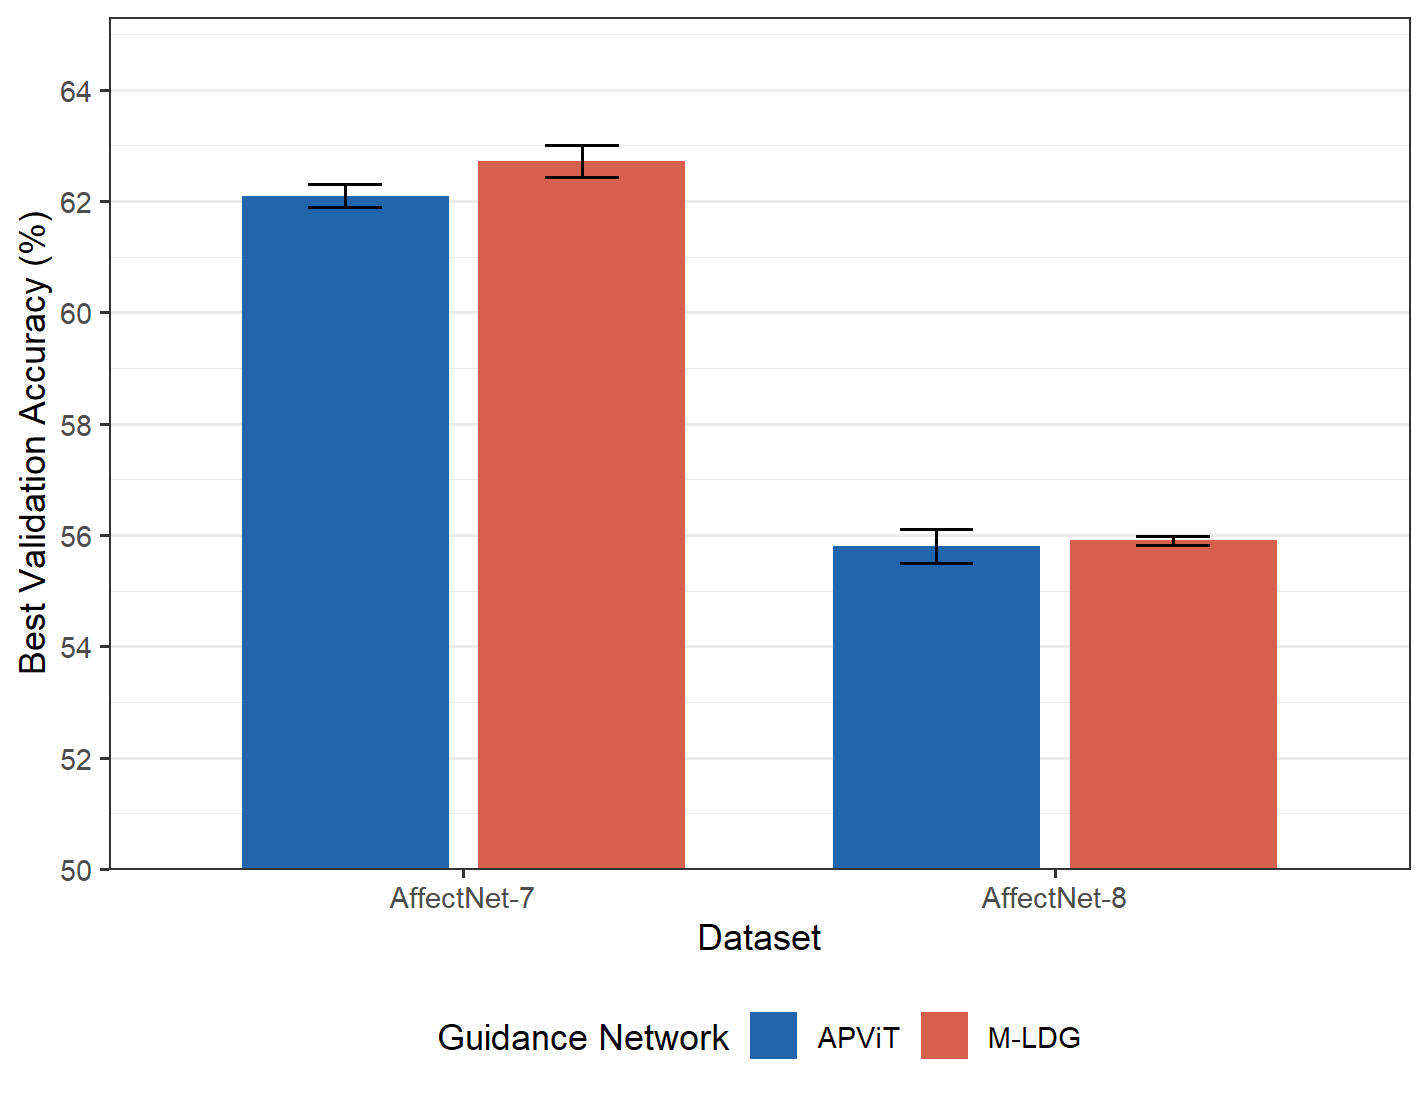
\includegraphics[width=1\columnwidth]{../images/chap_results/phase2comp.png}
    \caption[Phase II cell means bar chart]{Cell means for EfficientFace best validation accuracy under each guidance network and dataset condition in Phase II. Error bars indicate the range between the two replicates in each cell.}
    \label{fig:results-p2-bars}
\end{figure}

\subsection{Significance testing}
\label{section:results-phase2-significance}

Welch's t-tests were applied separately for each dataset to compare the mean accuracy of M-LDG-guided and APViT-guided EfficientFace, as specified in the \nameref{chapter:methodology} chapter.\\

For AffectNet-7, the mean accuracy was 62.71\% for M-LDG (SD = 0.404\%) and 62.10\% for APViT (SD = 0.303\%). The observed difference was +0.614 pp in favor of the M-LDG. The Welch t-test yielded $t(1.85) = -1.720$ with $p = 0.237$ and a 95\% confidence interval of $[-1.044,\ 2.272]$ pp. For AffectNet-8, the mean accuracy was 55.90\% for M-LDG (SD = 0.124\%) and 55.80\% for APViT (SD = 0.442\%). The observed difference was +0.100 pp in favor of the M-LDG. The Welch t-test yielded $t(1.16) = -0.308$ with $p = 0.804$ and a 95\% confidence interval of $[-2.917,\ 3.117]$ pp.\\

Neither comparison reached statistical significance. The wide confidence intervals spanning zero in both cases indicate that the direction of the difference cannot be established at the current sample size. With $n = 2$ replicates per cell, the Phase II tests are severely underpowered and can only detect very large effects; the failure to reach significance should be interpreted as inconclusive rather than as evidence of equivalence between M-LDG and APViT as guidance networks for EfficientFace.\\

\subsection{Hyperparameter optimization}
\label{section:results-phase2-optim}

Following the same Bayesian sweep procedure as Phase I, hyperparameter optimization was applied to two Phase II conditions: M-LDG with AffectNet-7 and APViT with AffectNet-8. Five 20-epoch sweep trials were conducted per combination, followed by 65-epoch confirmatory runs using the best identified configuration.\\

The optimized confirmatory runs achieved 62.29\% for M-LDG on AffectNet-7 and 55.01\% for APViT on AffectNet-8. These are lower than the corresponding Phase II baseline runs conducted with default hyperparameters, which achieved 63.00\% and 56.11\%, respectively. The differences represent decreases of -0.43 pp and -0.45 pp. Hyperparameter optimization in Phase II therefore produced a negative result: the default training configuration (learning rate 0.1, momentum 0.9, weight decay $10^{-4}$, LR factor 0.1, adjustment frequency 10) outperformed all optimized configurations identified by the sweep.\\

\section{Additional obtained metrics}
\label{section:results-metrics}

\subsection{Cross-phase accuracy progression}
\label{section:results-metrics-progression}

To summarize the accuracy gains at each stage of the proposed pipeline, Table \ref{tab:results-progression} presents the cross-phase accuracy progression from the unguided LDG baseline through to the final EfficientFace variants. This table directly addresses specific objective 3 from the \nameref{chapter:hypothesis-objectives} chapter, which calls for training two EfficientFace variants and studying their performance relative to the baseline and to each other.\\

\begin{table}[h!]
    \centering
    \begin{tabular}{@{}lrr@{}}
    \toprule
    \textbf{Stage} & \textbf{AffectNet-7} & \textbf{AffectNet-8} \\
    \midrule
    M-LDG baseline (C=False, ablation)             & 55.51 & 49.24 \\
    M-LDG + APViT guidance (C=True, ablation)      & 63.31 & 57.06 \\
    M-LDG (Phase I optimized)                    & \textbf{64.34} & \textbf{57.71} \\
    EfficientFace guided by M-LDG (Phase II)     & 63.00 & 55.99 \\
    EfficientFace guided by APViT (Phase II)     & 62.31 & 56.11 \\
    \midrule
    Published EfficientFace \cite{eff-face2021} & 63.70 & 59.89 \\
    Published APViT \cite{apvit2023}            & 66.91 & --- \\
    APViT trained from scratch                  & 64.2 & 57.31 \\
    \bottomrule
    \end{tabular}
    \caption[Cross-phase accuracy progression]{Accuracy (\%) at each stage of the proposed knowledge transfer pipeline for both AffectNet subsets. Published baselines from \cite{eff-face2021} and \cite{apvit2023} are provided for reference. We also present the performance of our own APViT model trained from scratch on AffectNet 7 and 8.}
    \label{tab:results-progression}
\end{table}

The unguided M-LDG baseline (C=False) achieved 55.51\% on AffectNet-7 and 49.24\% on AffectNet-8. Adding APViT knowledge distillation (C=True) raised accuracy to 63.31\% and 57.06\%, respectively. The M-LDG, after hyperparameter optimization, reached 64.34\% (AffectNet-7) and 57.71\% (AffectNet-8). EfficientFace trained with M-LDG-generated soft labels achieved 63.00\% (AffectNet-7) and 55.99\% (AffectNet-8), while EfficientFace trained with APViT-generated soft labels achieved 62.31\% and 56.11\%. For reference, the original EfficientFace authors report 63.7\% on AffectNet \cite{eff-face2021} and the APViT teacher used in this study reports 66.91\% on AffectNet \cite{apvit2023}.\\

\subsection{Per-class behavior}
\label{section:results-metrics-perclass}

In addition to the top-1 accuracy response variable, per-class validation confusion matrices were logged for all runs via WandB. We report here the confusion matrices for the best M-LDG-guided EfficientFace variants obtained in Phase II: the AffectNet-7 model (63\% best accuracy) and the AffectNet-8 model (55.99\% best accuracy). These matrices capture the distribution of correct and incorrect predictions across expression classes and complement the main accuracy reported throughout this chapter.\\

Figure \ref{fig:results-cm-an7} shows the normalized confusion matrix for the best M-LDG-guided EfficientFace on AffectNet-7 and figure \ref{fig:results-cm-an8} shows the corresponding matrix for AffectNet-8.\\

\begin{figure}[h!]
    \centering
    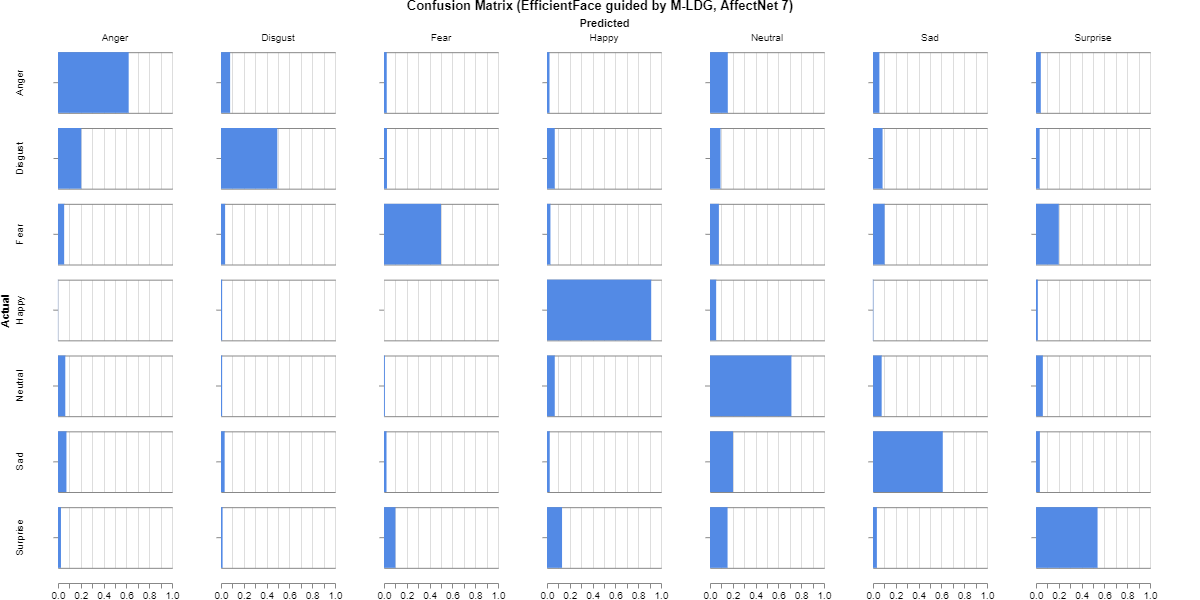
\includegraphics[width=1\columnwidth]{../images/chap_results/7classconf.png}
    \caption[Confusion matrix: M-LDG EfficientFace on AffectNet-7]{Normalized confusion matrix for the best M-LDG-guided EfficientFace variant on AffectNet-7. Rows represent true classes; columns represent predicted classes. Values indicate the fraction of samples in each true-class row assigned to each predicted class.}
    \label{fig:results-cm-an7}
\end{figure}

\begin{figure}[h!]
    \centering
    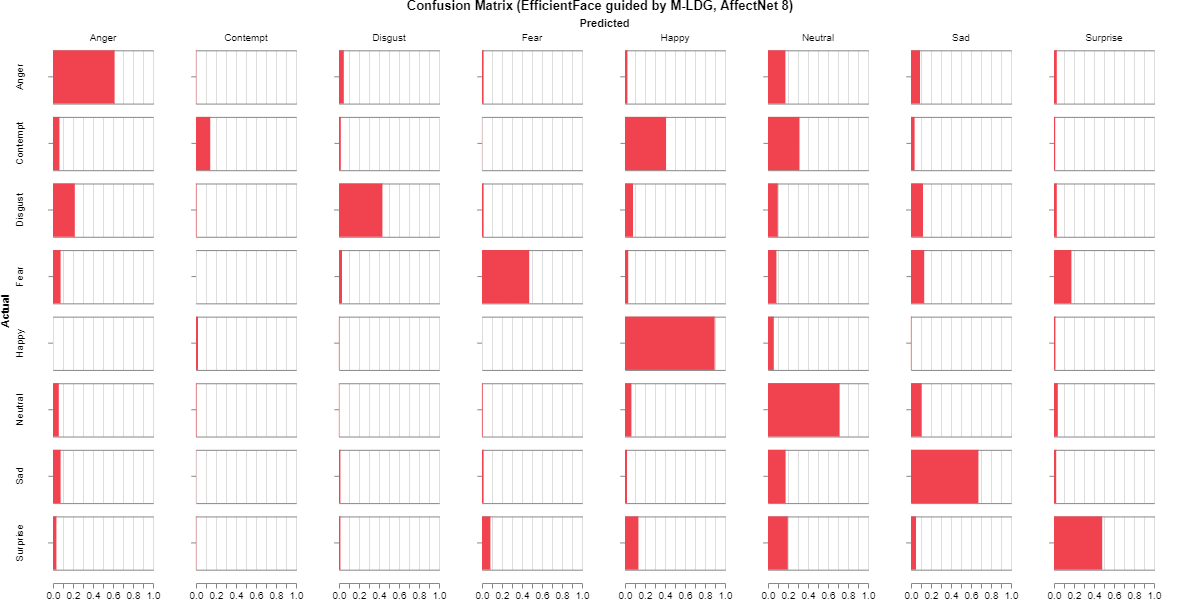
\includegraphics[width=1\columnwidth]{../images/chap_results/8classconf.png}
    \caption[Confusion matrix: M-LDG EfficientFace on AffectNet-8]{Normalized confusion matrix for the best M-LDG-guided EfficientFace variant on AffectNet-8, including the contempt class. Rows and columns follow the same convention as figure \ref{fig:results-cm-an7}.}
    \label{fig:results-cm-an8}
\end{figure}

\subsection{Per-class and macro-averaged metrics}
\label{section:results-metrics-classmetrics}

Beyond the top-1 accuracy response variable, we computed per-class and macro-averaged classification metrics for the five pipeline stages of table \ref{tab:results-progression} on both AffectNet subsets, derived from the same logged confusion matrices used in section \ref{section:results-metrics-perclass}. These metrics were not subjected to the formal statistical analysis applied to top-1 accuracy in Phases I and II and are reported here as descriptive summaries only. Table \ref{tab:results-perclass-acc} reports per-class recall, and table \ref{tab:results-macro} reports the macro-averaged precision, recall, and F1 score alongside top-1 accuracy for all ten trained models.\\

\begin{table}[h!]
    \centering
    \footnotesize
    \resizebox{\linewidth}{!}{%
    \begin{tabular}{@{}lrrrrr@{}}
    \toprule
    \multicolumn{6}{c}{\textbf{AffectNet-7}} \\
    \cmidrule(lr){2-6}
    \textbf{Emotion} & \textbf{M-LDG base} & \textbf{M-LDG+APViT} & \textbf{M-LDG optim.} & \textbf{EF+APViT} & \textbf{EF+M-LDG} \\
    \midrule
    Anger    & 0.562 & \textbf{0.660} & 0.654 & 0.656 & 0.622 \\
    Disgust  & 0.282 & 0.450 & \textbf{0.514} & 0.436 & 0.506 \\
    Fear     & 0.440 & \textbf{0.540} & 0.538 & 0.498 & 0.520 \\
    Happy    & \textbf{0.936} & 0.914 & 0.908 & 0.928 & 0.914 \\
    Neutral  & \textbf{0.784} & 0.726 & 0.716 & 0.700 & 0.704 \\
    Sad      & 0.518 & \textbf{0.642} & 0.634 & 0.622 & 0.618 \\
    Surprise & 0.364 & 0.500 & \textbf{0.540} & 0.522 & 0.526 \\
    \midrule
    \multicolumn{6}{c}{\textbf{AffectNet-8}} \\
    \cmidrule(lr){2-6}
    \textbf{Emotion} & \textbf{M-LDG base} & \textbf{M-LDG+APViT} & \textbf{M-LDG optim.} & \textbf{EF+APViT} & \textbf{EF+M-LDG} \\
    \midrule
    Anger    & 0.564 & 0.638 & \textbf{0.642} & \textbf{0.642} & 0.612 \\
    Contempt & 0.004 & 0.134 & \textbf{0.186} & 0.124 & 0.164 \\
    Disgust  & 0.286 & 0.460 & \textbf{0.466} & 0.450 & 0.452 \\
    Fear     & 0.444 & 0.504 & \textbf{0.522} & 0.502 & 0.478 \\
    Happy    & \textbf{0.950} & 0.920 & 0.894 & 0.908 & 0.898 \\
    Neutral  & \textbf{0.776} & 0.682 & 0.714 & 0.684 & 0.714 \\
    Sad      & 0.566 & \textbf{0.702} & 0.682 & 0.686 & 0.666 \\
    Surprise & 0.348 & \textbf{0.524} & 0.510 & 0.492 & 0.494 \\
    \bottomrule
    \end{tabular}%
    }
    \smallskip
    \caption[Per-class recall by pipeline stage]{Per-class recall for the five pipeline stages of table \ref{tab:results-progression} on both AffectNet subsets.}
    \label{tab:results-perclass-acc}
\end{table}

\begin{table}[h!]
    \centering
    \footnotesize
    \resizebox{\linewidth}{!}{%
    \begin{tabular}{@{}lrrrrr@{}}
    \toprule
    \multicolumn{6}{c}{\textbf{AffectNet-7}} \\
    \cmidrule(lr){2-6}
    \textbf{Metric} & \textbf{M-LDG base} & \textbf{M-LDG+APViT} & \textbf{M-LDG optim.} & \textbf{EF+APViT} & \textbf{EF+M-LDG} \\
    \midrule
    Top-1 Acc.\ (\%) & 55.51 & 63.31 & \textbf{64.34} & 62.31 & 63.00 \\
    Precision              & 0.626 & 0.653 & \textbf{0.658} & 0.647 & 0.643 \\
    Recall             & 0.555 & 0.633 & \textbf{0.643} & 0.623 & 0.630 \\
    F1                 & 0.543 & 0.629 & \textbf{0.641} & 0.618 & 0.627 \\
    \midrule
    \multicolumn{6}{c}{\textbf{AffectNet-8}} \\
    \cmidrule(lr){2-6}
    \textbf{Metric} & \textbf{M-LDG base} & \textbf{M-LDG+APViT} & \textbf{M-LDG optim.} & \textbf{EF+APViT} & \textbf{EF+M-LDG} \\
    \midrule
    Top-1 Acc.\ (\%) & 49.24 & 57.06 & \textbf{57.71} & 56.11 & 55.99 \\
    Precision              & \textbf{0.641} & 0.634 & 0.628 & 0.625 & 0.622 \\
    Recall             & 0.492 & 0.571 & \textbf{0.577} & 0.561 & 0.560 \\
    F1                 & 0.454 & 0.549 & \textbf{0.562} & 0.540 & 0.543 \\
    \bottomrule
    \end{tabular}%
    }
    \smallskip
    \caption[Macro-averaged validation metrics by pipeline stage]{Macro-averaged precision, recall, and F1 score with the corresponding top-1 validation accuracy (\%) for the five pipeline stages of table \ref{tab:results-progression} on both AffectNet subsets. Macro averages weight every class equally regardless of its sample count.}
    \label{tab:results-macro}
\end{table}

\subsection{Model complexity}
\label{section:results-metrics-complexity}

Table \ref{tab:results-complexity} reports the parameter and MFLOPs (floating-point operations) counts for the four architectures involved in the proposed pipeline alongside the best top-1 validation accuracy each achieved on AffectNet-7. Counts were computed using the \texttt{thop} library \cite{lyken17_thop}, with each multiply-accumulate (MAC) operation counted as one FLOP. The 7-class and 8-class variants of each model differ only in their final classification head, so the 7-class figures serve as representative values.\\

\begin{table}[h!]
    \centering
    \begin{tabular}{@{}lrrr@{}}
    \toprule
    \textbf{Model} & \textbf{Best Acc.\ (\%)} & \textbf{Params (M)} & \textbf{MFLOPs} \\
    \midrule
    M-LDG                                & 64.34 & 56.43 &  6334.4 \\
    EfficientFace (Phase II)                        & 63.00 &  1.28 &   158.6 \\
    Original LDG \cite{eff-face2021}   & ---   & 23.52 &  4131.7 \\
    APViT \cite{apvit2023}          & 66.91 & 65.06 & 12400.1 \\
    \bottomrule
    \end{tabular}
    \smallskip
    \caption[Model complexity summary]{Best AffectNet-7 accuracy, parameter count (in millions), and MFLOPs for the four architecture families under study. M-LDG variants share identical complexity, as do all EfficientFace variants. Original LDG accuracy on AffectNet is not reported in \cite{eff-face2021}.}
    \label{tab:results-complexity}
\end{table}

\subsection{Interpretability}
\label{section:results-metrics-cam}

To provide evidence of the spatial attention patterns learned by the main networks in our study, we apply class activation maps (CAMs) \cite{cams2016}. CAM visualizations highlight the image regions that contributed most strongly to the network's predicted class, offering a spatial perspective on model behavior that complements the quantitative accuracy metrics reported in the preceding sections.\\

Figure \ref{fig:results-cam} presents a grid of CAM visualizations for four of the five networks presented in the cross phase comparison (see table \ref{tab:results-progression}).\\

\begin{figure}[h!]
    \centering
    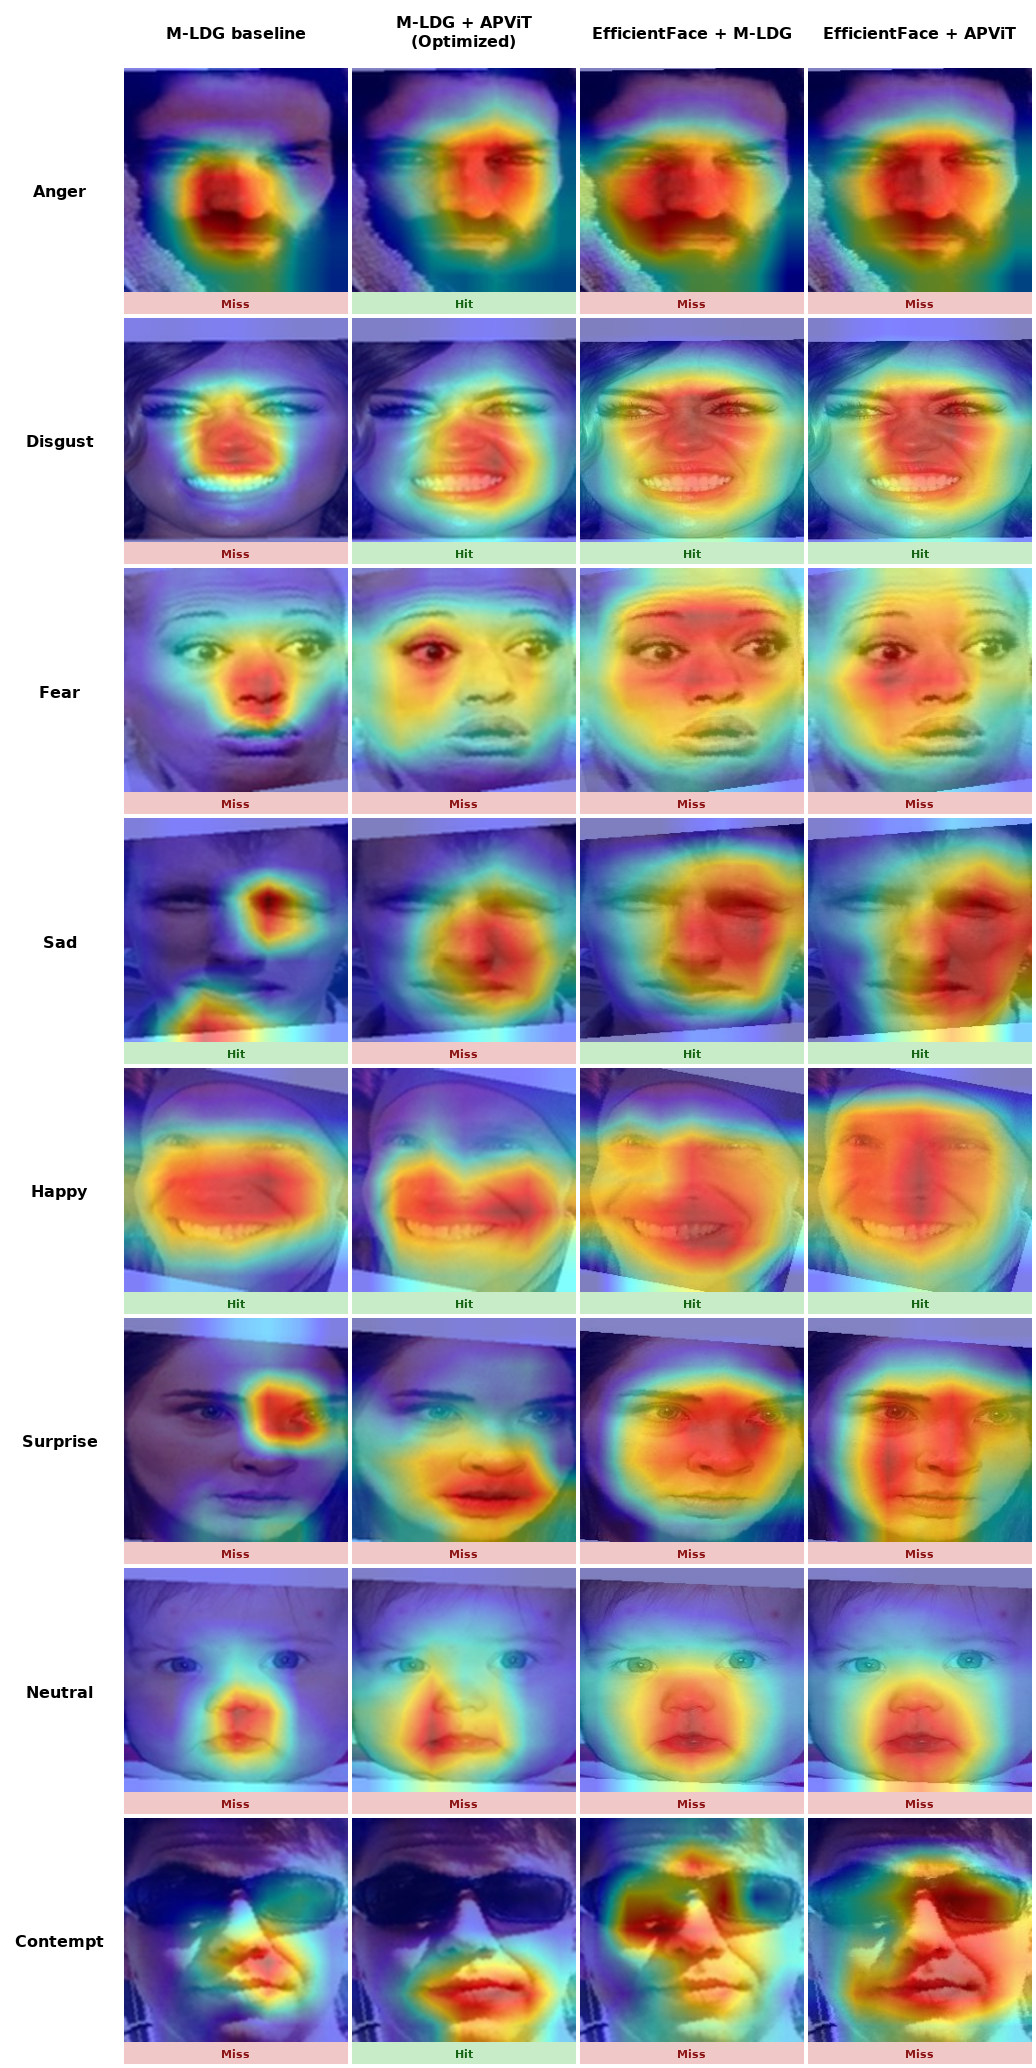
\includegraphics[width=0.65\columnwidth]{../images/chap_results/mixedcamgrid.png}
    \caption[CAM visualizations]{Class activation map (CAM) visualizations for the four of the five main networks used in the cross phase comparison (see table \ref{tab:results-progression}). Each panel shows one validation sample with the model's spatial attention overlaid. Warmer colors indicate higher activation. Hit and miss labels under each image indicate if the sample is correctly or incorrectly classified.}
    \label{fig:results-cam}
\end{figure}

\newpage

%Disussion

\chapter{Discussion}
\epigraph{``To consult the statistician after an experiment is finished is often merely to ask him to conduct a post mortem examination. He can perhaps say what the experiment died of.''}{\vspace{10pt}Ronald A. Fisher}
\label{chapter:discussion}

\newpage

This chapter presents the analysis and discussion of the findings reported in the previous chapter. We interpret the Phase I ablation and Phase II experimental results in light of the hypothesis and specific objectives defined in the \nameref{chapter:hypothesis-objectives} chapter, following the statistical procedures described in the \nameref{chapter:methodology} chapter. The discussion is organized around five themes: the rejection of the main hypothesis, the mechanics of the two-hop knowledge transfer chain, the reasons why the individual LDG enhancements failed to propagate to the student network, a set of auxiliary observations, and a final synthesis that integrates these threads.

\section{Revisiting the hypothesis}
\label{section:discussion-hypothesis}

The main hypothesis of our study reads: \textit{``Training EfficientFace with a label distribution generator enhanced with one or more of: FER pretrained backbone weights, local-global feature extraction modules, and/or vision transformer guidance, should increase its facial expression recognition accuracy on the AffectNet dataset when compared to the original baseline.''}\\

The evidence does not support this claim. The best-performing enhanced configuration, EF + M-LDG (EfficientFace trained with M-LDG-generated soft labels), achieved 63.00\% on AffectNet-7 (AN-7) and 55.99\% on AffectNet-8 (AN-8), while the published EfficientFace baseline \cite{eff-face2021} reports 63.70\% and 59.89\% on the same subsets. The alternative enhanced configuration, EF + APViT, similarly achieved 62.31\% (AN-7) and 56.11\% (AN-8), remaining below the published reference. Across both AffectNet subsets and both EfficientFace configurations tracked in Table~\ref{tab:results-p2-cells}, accuracy remained below the published reference. \textbf{We therefore reject the hypothesis}. The following sections will explore the reasons why this happened.

\section{The two-hop knowledge transfer chain}
\label{section:discussion-transfer-chain}

This section examines the two hops of the knowledge transfer chain and identifies the possible causes responsible for the asymmetric outcomes observed across hops.\\

\subsection{Asymmetric transfer across the two hops}
\label{section:discussion-dp2}

The transfer chain runs from APViT (teacher, 65.06M params) through the modified label distribution generator (M-LDG, intermediary, 56.43M params) to EfficientFace (student, 1.28M params). The first hop from APViT to M-LDG proved highly effective: APViT itself achieves 64.2\% and 57.31\% on AffectNet-7 and AffectNet-8 respectively; the APViT-guided M-LDG achieves 64.34\% on AffectNet-7, and 57.71\% on AffectNet-8 (see Table~\ref{tab:results-progression}). This means that in the first phase the student network was able to maintain the teacher's performance while being around 13\% smaller in terms of parameters. The second hop, from M-LDG to EfficientFace via label distribution learning, did not exhibit the same improvement.\\

EfficientFace trained with M-LDG-generated distributions (EF + M-LDG) achieved 63\% and 55.99\% on AffectNet-7 and AffectNet-8 respectively, drops of 1.34 pp and 1.81 pp below the M-LDG's own accuracy. This is in direct contrast to the original EfficientFace result, where the label distribution learning-trained (LDL) student surpassed its LDG teacher \cite{eff-face2021}. That observation established the expectation that LDL produces a beneficial effect sufficient to overcome the student's capacity disadvantage. In the present phase II setup, this expectation was not met.\\

We attribute the failure to a pronounced difference in capacity between the M-LDG and EfficientFace. The original EfficientFace paper \cite{eff-face2021} employed a LDG of 23.52M parameters, a scale far closer to EfficientFace's own parameter count. The M-LDG, at 56.43M parameters and 6334.4 MFLOPs, produces a ratio of approximately 44 to 1 relative to EfficientFace's 1.28M parameters and 158.6 MFLOPs (Table~\ref{tab:results-complexity}). This expanded capacity gap is a key structural difference between the present setup and the original, and we argue it is responsible for the transfer asymmetry. The study by Mirzadeh et al. \cite{mirzadeh2020takd} on knowledge distillation via intermediate network assistance supports this claim as well. In their study, the authors found that large gaps in student and teacher sizes can significantly degrade performance.

\subsection{Teacher-agnosticism of EfficientFace}
\label{section:discussion-dp3}

Phase II found no statistically significant difference between M-LDG and APViT guidance on EfficientFace outcomes (Welch t-test $p = 0.237$ on AffectNet-7 and $p = 0.804$ on AffectNet-8), with 95\% confidence intervals spanning zero on both subsets (Table~\ref{tab:results-p2-cells}; section~\ref{section:results-phase2-significance}). The G factor difference was a modest +0.357 pp in favor of M-LDG, and the two conditions differed by less than one percentage point on both datasets, with per-class recall and F1 gaps of at most 0.03 (Table~\ref{tab:results-perclass-acc}). This result is best read as inconclusive rather than as evidence of equivalence: the comparison rested on $n = 2$ replications per cell, leaving the test statistically underpowered.\\

This result carries a double-edged interpretation. One positive reading of the result is that a computationally lighter intermediary can replace the full APViT transformer as the teacher signal during EfficientFace training without producing a meaningfully inferior student network, preserving the training-pipeline efficiency advantage that comes from avoiding the heavier APViT teacher. The negative reading, however, is that the higher performance of the M-LDG at the teacher level is downstream-irrelevant: an improvement of 7.889 pp in teacher accuracy failed to propagate into statistically distinguishable gains in the student network, so the training cost incurred by enhancements to the M-LDG yield no visible benefit in the final deployed model.\\

A possible explanation for this outcome centers on the relative sizes of the three networks. M-LDG and APViT are comparable in scale to each other, yet both are substantially larger than EfficientFace (see Table~\ref{tab:results-complexity}). If the capacity gap between each teacher and the student is the dominant constraint on knowledge transfer, then the comparatively small size difference between the two teachers becomes secondary: neither network is well-positioned to bridge the gap into EfficientFace effectively, and substituting one for the other leaves the student's learned representations essentially unchanged. This explanation is inferential, but it is consistent with the near-identical per-class profiles observed in Table~\ref{tab:results-perclass-acc}.

\section{Effectiveness of the LDG enhancements}
\label{section:discussion-enhancements}

This section examines why enhancements A (pretrained backbone weights) and B (local-global feature extraction modules) did not translate into improved M-LDG accuracy; the dominant role of enhancement C is analyzed in section~\ref{section:discussion-factorc}. The focus here is on the internal training dynamics of the M-LDG rather than the downstream knowledge transfer chain analyzed in the previous section.

\subsection{Negligible effects of factors A and B}
\label{section:discussion-factorab}

The phase I ablation study confirms factor C as the only statistically significant booster of M-LDG accuracy in this setup (Table~\ref{tab:results-anova}). Before drawing conclusions, we note that the standard deviation across all conditions ranged from 0.08 to 0.25 pp (Table~\ref{tab:results-p1-effects}), indicating that the experimental measurements are  precise. The negligible effects of A and B are therefore reliable findings rather than measurement artifacts obscured by noise.\\

We attribute the negligible effect of factor B to a structural mismatch between the origin of the local-global modules and the network into which they are inserted. The GL modules were originally designed for EfficientFace, a more shallow network whose reduced depth makes explicit local-global feature extraction a meaningful architectural addition \cite{eff-face2021}. Transplanting them into a ResNet-50 backbone places them inside a network that is already deep enough to  extract these same representations across its numerous layers. We therefore argue that a mechanism tailored for a shallow network loses its effectiveness when embedded in a substantially deeper one. Nonetheless, a visual comparison of the activation patterns (see Figure~\ref{fig:results-cam}) suggests that in spite of its lower accuracy, the EfficientFace variants that use GL modules do a better job of drawing attention towards the correct regions than the M-LDG variants that do not. There is one caveat regarding this interpretation for the contempt class, which will be discussed in section~\ref{section:discussion-auxiliary}.\\

The negligible effect of factor A is best understood by examining which parts of the M-LDG network actually receive FER-pretrained initialization. The APViT-derived weights cover only the first three stages of the IR50 backbone \cite{deng2019ir50}; the fourth stage and the classification head are not pretrained on FER and are instead initialized with weights from the face recognition pretraining on MS-Celeb-1M \cite{guo2016msceleb}. The richer, FER-specific knowledge encoded in the early stages therefore does not extend to the network's higher-level layers. Because the upper stage must still learn high-level FER representations almost from scratch, the benefit of low-level FER-pretrained initialization is insufficient to guide learning at the levels where it matters most.

\subsection{Evidence for APViT's guidance and regularization role}
\label{section:discussion-factorc}

Our ablation study provides strong evidence in favor of APViT's effectiveness as a teacher network. Its presence improved M-LDG label distribution quality by +7.889 pp (see Table~\ref{tab:results-anova}), a large and highly significant effect. Following hyperparameter optimization, the M-LDG reached 64.34\% on AffectNet-7 and 57.71\% on AffectNet-8, an improvement over the baseline of +8.83 pp and +8.47 pp respectively (Table~\ref{tab:results-progression}).\\

A secondary observation can be made on the effect of APViT guidance on overfitting. As documented in section~\ref{section:results-phase1-curves} and illustrated in Figure~\ref{fig:results-p1-curves}, M-LDG configurations without APViT guidance (C$-$) exhibited severe overfitting. The observed pattern places these configurations at high levels of training accuracy but  low levels of validation accuracy. Whereas configurations with APViT guidance (C$+$) exhibit the opposite pattern, with higher validation accuracy and lower training accuracy. This reduction reveals a dual role for the label distribution learning (LDL) loss. Its primary role is what motivated its inclusion: the LDL loss causes the M-LDG to produce soft label distributions that encode the teacher's uncertainty across emotion classes. Its secondary role, however, is that of an implicit regularizer: by constraining the M-LDG's outputs to remain close to APViT's more nuanced predictions, the LDL loss substantially reduces overfitting and steers the model toward a more generalizable function.

\section{Auxiliary observations}
\label{section:discussion-auxiliary}

This section provides complementary observations to the main discussion points exposed above. While not central to our study, they provide additional insights that could serve as a starting point for future work.

\subsection{Challenge of the contempt class}
\label{section:discussion-a3}

Factor D (AffectNet-8 versus AffectNet-7) imposed an accuracy penalty of $-6.297$ pp across all M-LDG configurations (Table~\ref{tab:results-p1-effects}), reflecting the added difficulty of the eight-class subset. Contempt recall collapsed to 0.004 for the LDG baseline and recovered to only 0.186 for the optimized M-LDG (Table~\ref{tab:results-perclass-acc}), indicating that this class remains nearly undetectable across all configurations. Contempt is the least frequent class in AffectNet-8 and also among the most challenging to label reliably, and its near-zero recall is likely one of the causes of the large gap between our best EfficientFace result (55.99\%) and the published AffectNet-8 baseline (59.89\%).\\

On a similarly interesting note, we have some light evidence for the contempt class being predicted by the mouth region. From the employed models, we note that the optimized M-LDG is slightly better than the EfficientFace at identifying contempt (M-LDG recall 0.186 vs EfficientFace recall 0.164). We complement this observation with the activation maps for the contempt class. The single sample shown in Figure~\ref{fig:results-cam} shows the M-LDG focusing on the mouth region to correctly classify the image. Analyzing a wider set of samples classified by the M-LDG we observe that correctly labeled images tend to focus almost exclusively on the mouth region, whereas incorrectly classified images tend to focus on other regions. This is shown in Figure~\ref{fig:discussion-a3-activations}. This observation should not be taken as definitive given the lack of backing quantitative evidence. Still, it is an interesting pattern that could be further explored in another study.

\begin{figure}[h!]
    \centering
    \begin{minipage}{0.49\columnwidth}
        \centering
        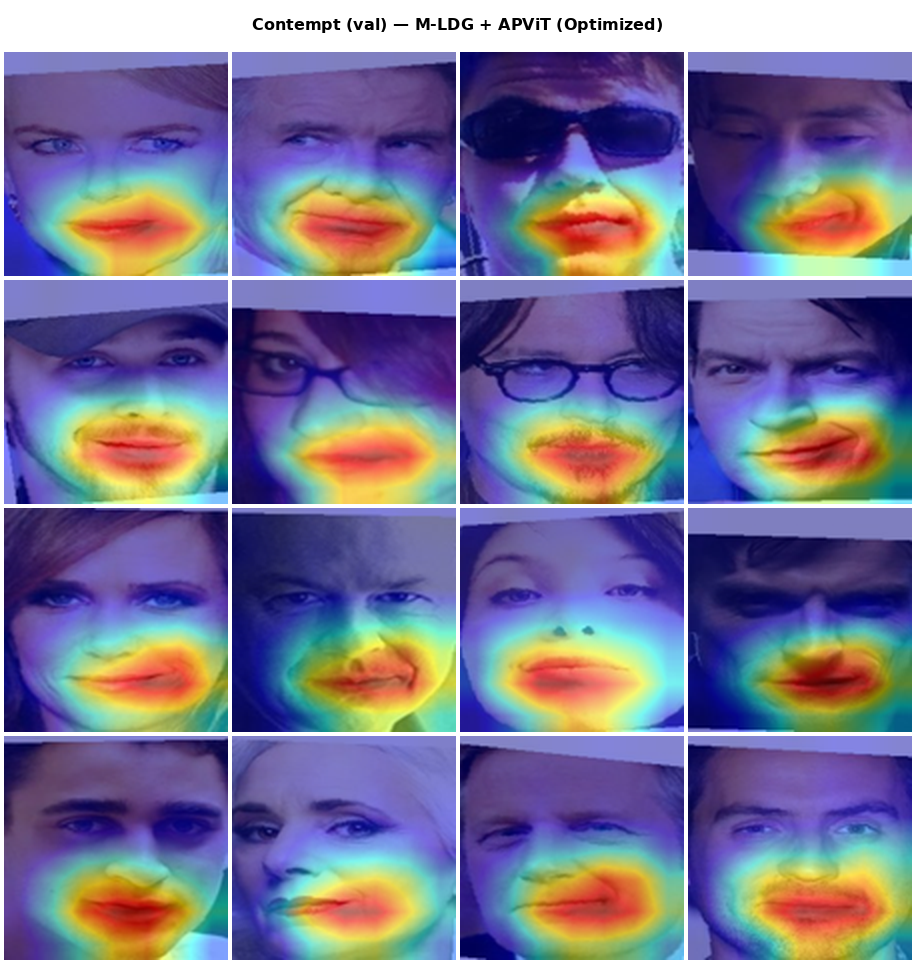
\includegraphics[width=\linewidth]{../images/chap_discussion/contempthits.png}
    \end{minipage}\hfill
    \begin{minipage}{0.49\columnwidth}
        \centering
        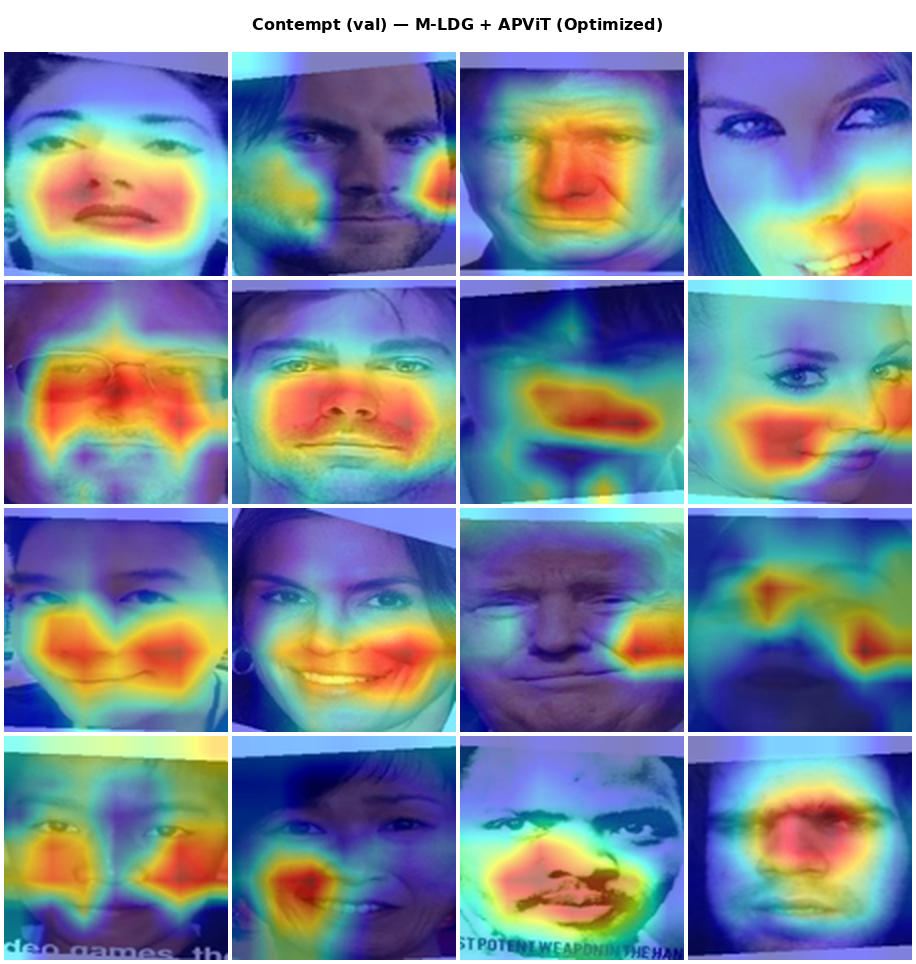
\includegraphics[width=\linewidth]{../images/chap_discussion/contemptmisses.png}
    \end{minipage}
    \caption[M-LDG activation maps for the contempt class]{Activation maps for the contempt class on samples classified by the optimized M-LDG. Left: correctly classified samples; right: incorrectly classified samples.}
    \label{fig:discussion-a3-activations}
\end{figure}

\subsection{Macro-averaged precision, recall, and F1 patterns}
\label{section:discussion-macro-metrics}

Table~\ref{tab:results-macro} extends Table~\ref{tab:results-progression} with macro-averaged precision, recall, and F1 across all five configurations on AffectNet-7 and AffectNet-8. On AffectNet-7, recall and F1 mirror the top-1 accuracy: M-LDG base achieves recall 0.555 and F1 0.543; the optimized M-LDG peaks at 0.643 and 0.641. Precision is comparatively stable across configurations (0.626 to 0.658). This data suggests that the progression in Table~\ref{tab:results-progression} is not an artifact of accuracy as a metric choice.\\

On AffectNet-8, the M-LDG base records the highest precision (0.641) despite the lowest recall (0.492). We attribute this inversion to contempt-class suppression (section~\ref{section:discussion-a3}), i.e. rarely predicting a class yields few false positives for it, which inflates its precision contribution to the macro average. As APViT guidance broadens the distribution of predictions, false positives accumulate in suppressed categories, pulling precision to 0.628 for the optimized M-LDG while recall rises by 0.085. Precision alone is therefore a misleading indicator in the imbalanced AffectNet-8 setting.\\

The near-identical metric profiles of EF+APViT and EF+M-LDG corroborate the teacher-agnosticism finding from section~\ref{section:discussion-dp3}. The largest single-metric gap between the two across both datasets is 0.009 (AffectNet-7 F1: 0.618 vs. 0.627; Table~\ref{tab:results-macro}). On AffectNet-8, all three measures differ by at most 0.003. These margins are consistent with the phase II results and reinforce the interpretation that substituting one teacher for the other leaves the student's learned representations nearly indistinguishable.

\subsection{Implementation constraints and their downstream effects}
\label{section:discussion-implementation-constraints}

Because publicly available AffectNet-pretrained weights for APViT \cite{apvit2023} did not exist at the time of this study, the network was trained from scratch on AffectNet, as described in chapter \nameref{chapter:design}. This model did not reach the same level of performance as the published one, and we argue this likely introduced a performance ceiling for APViT in its role as teacher network. The downstream consequences of this ceiling extend across most experimental conditions: it affects all M-LDG variants trained with APViT guidance or FER pre-trained weights (factors A and C), it indirectly affects EfficientFace variants trained with M-LDG-generated distributions, and it affects the EfficientFace variant trained with APViT guidance directly.\\

We are careful to limit this claim. The from-scratch training constraint defines a possible ceiling of the pipeline, but it does not displace the capacity bottleneck as the likely primary culprit of the transfer failure. The from-scratch limitation is therefore best understood as a contributing factor that bounds how high the pipeline's ceiling can reach, rather than as the root cause of why the student did not exceed the published baseline.\\

We attribute the lower accuracy of the in-house trained APViT to the difficulty in replicating the exact training procedure used in the original paper. The public APViT codebase \cite{apvit2023} was oriented toward training on RAF-DB, and adapting it to AffectNet required non-trivial modifications to data loading, preprocessing, and training procedures. The EfficientFace codebase \cite{eff-face2021} is similarly RAF-DB-oriented by default, and its adaptation is a likely source of noise that is hard to design for. These modifications introduce sources of experimental uncertainty that are difficult to fully quantify, and they provide additional context for interpreting the reproducibility gap with the published baseline discussed in section~\ref{section:discussion-hypothesis}.

\subsection{Hyperparameter optimization failure in Phase II}
\label{section:discussion-p2-hpo}

Despite using the same set of hyperparameters and levels as Phase I, the procedure did not yield any improvement over the default hyperparameters in Phase II. On the contrary, the attempted optimized runs performed approximately as well as the default configuration. This result is consistent with the findings of the Phase II comparison runs, which also did not yield any improvement over the default hyperparameters.\\

A likely explanation for this outcome is that the wide gap between teacher and student network capacities mentioned before has a performance-limiting effect. This means that even with varying sets of hyperparameters, the performance of the student network is capped at approximately the same level that was reached by the initial Phase II models. Further exploration of the hyperparameter space fails to yield any improvement due to it being constrained by the capacity gap. In all likelihood, the default configuration was already close to the optimal one for this setup only because of this limitation.

\section{Synthesis}
\label{section:discussion-synthesis}

The central takeaway of this study is that enhancing the intermediary teacher worked, but that success did not carry through to the final student network. APViT guidance lifted the M-LDG to 64.34\% on AffectNet-7 and 57.71\% on AffectNet-8, providing a substantial gain driven not just by richer soft labels, but by the implicit regularization effect that kept C$-$ configurations from overfitting badly. The pipeline, at that level behaved as intended. \\

However, it was unable to overcome the scale mismatch at the second hop. A capacity ratio of roughly 44 to 1 between the M-LDG and EfficientFace is too wide for label distribution learning to bridge. The original EfficientFace paper demonstrated that a student can surpass its teacher through LDL, but that result assumed a far more modest gap between the two networks. Stretching that gap to the degree present here appears to neutralize whatever advantage the richer soft labels provide, and the near-identical outcomes of EF+M-LDG and EF+APViT reinforce the point: with a large scale difference, swapping one teacher for another does not make a significant difference in the student.\\

FER-pretrained weights and GL modules (factors A and B) tell a related story about transplanting mechanisms outside their intended context. When embedding the GL modules designed for the shallow EfficientFace into a deep ResNet-50, their contribution becomes redundant. FER-pretrained initialization only reached the first three backbone stages, leaving the upper layers, where high-level expression representations form, without any FER-specific grounding. Neither enhancement was wrong in principle; both were simply mismatched to the architecture they were applied to.\\

The from-scratch APViT training constraint sits on top of all of this as an additional limiting factor. It is worth being precise about what role it plays: it lowered the ceiling of the teacher signal, but it did not cause the transfer failure. A stronger APViT would have produced a stronger M-LDG, and possibly a marginally better student, but not necessarily one that clears the published baseline. The capacity bottleneck remains regardless of this limitation.\\

The more productive direction for future work is probably not to keep refining the teacher, but to address the gap directly. Mirzadeh et al. \cite{mirzadeh2020takd} suggest that an intermediate-capacity assistant network can bridge large student-teacher size differences more effectively than direct distillation; that approach seems a natural fit here. Alternatively, techniques that sharpen or re-weight the soft label distributions before passing them to the student might help preserve more of the teacher signal across the gap. Either way, the lesson from this pipeline is that the bottleneck is structural, and architectural interventions that ignore it are unlikely to move the needle. 
%Conclusions and future work
\chapter{Conclusions and Future Work}
\epigraph{``We can only see a short distance ahead, but we can see plenty there that needs to be done.''}{\vspace{10pt}Alan M. Turing}
\label{chapter:conclusions-fw}

\newpage

This chapter distills the main findings of this research, drawing on the experimental evidence reported in the \nameref{chapter:results} chapter and the interpretive analysis developed in the previous chapter.

\section{Conclusions}

\begin{itemize}
	\item The hypothesis is rejected: no enhanced EfficientFace configuration surpassed the published AffectNet baseline. The proposed variant, EfficientFace trained with soft labels from the M-LDG, reached 63\% on AffectNet-7 and 55.99\% on AffectNet-8 against a published reference of 63.70\% and 59.89\%.

	\item APViT guidance substantially improved the M-LDG, adding roughly 8 to 9 percentage points and lifting it to 64.34\% on AffectNet-7 and 57.71\% on AffectNet-8, confirming that the first hop of the two-stage transfer pipeline behaved as intended.

	\item The second hop of the transfer pipeline was not able to bridge the accuracy gap between the M-LDG and EfficientFace. We attribute this to the large capacity (in millions of parameters) gap between the two networks. With a ratio of approximately 44 to 1, the label distribution learning approach hits a bottleneck. This aligns with existing literature on knowledge distillation when using networks with large differentials \cite{mirzadeh2020takd}.

	\item FER-pretrained backbone weights and local-global feature extraction modules both contributed negligibly to M-LDG accuracy in Phase I, though for different reasons: the former's pretrained weights covered only the first three backbone stages, leaving the upper layers and classification head without FER-specific initialization, while the latter's modules were designed for the shallow EfficientFace architecture and became redundant in the deeper IR50.

	\item Replacing the full APViT transformer with the lighter M-LDG as the direct teacher for EfficientFace in Phase II produced no statistically significant difference in student accuracy, suggesting that the computationally lighter intermediary can stand in for the heavier model without a meaningful loss in transfer quality; this finding remains tentative, however, given the limited number of experimental runs available for that comparison.
\end{itemize}


\section{Future Work}

\begin{itemize}


	\item Reducing the M-LDG network size to better approximate the capacity of EfficientFace could improve the second hop of the transfer pipeline. Another approach could be to discard the APViT component and instead replicate the study with another network acting as intermediary. This keeps in line with the evidence from Mirzadeh et al.'s \cite{mirzadeh2020takd} where carefully selected intermediary network sizes can improve the transfer efficiency.

	\item The contempt class warrants deeper investigation: its recall remained near zero for the ablation baseline and recovered only partially under the optimized M-LDG, and the tentative observation that contempt recognition relies predominantly on the mouth region should be validated with quantitative, region-weighted evidence.

	\item Revisiting the pipeline with publicly available AffectNet-pretrained weights, should provide a better gain in performance. This could be with the same APViT network or choosing another similar method that is confirmed to have the weights available.
	
	\item The lack of statistical power in the phase II experiments warrants a larger sample size. This could be achieved by introducing additional factors into the experimental design like use of upscaling and teacher network size. This could serve to better approximate the hard limit of the knowledge transfer pipeline as well as finding better configurations for the second hop. Additionally, prescinding from the already successful Phase I study could free up resources for additional replications in the second phase, increasing the statistical power of the study.

\end{itemize}

%Appendix

\chapter{Appendixes}
\label{chapter:appendixes}

\newpage

This section lists the public repositories and experiment-tracking resources used to implement and execute the experimental design.\\

\section{Source Code}
\label{deliverable:source-code}

\textbf{Main code repository:} The primary repository for this thesis contains the modified LDG and EfficientFace implementations, dataset preprocessing scripts, and Jupyter notebooks for experiment execution and hyperparameter optimization. It is available at \url{https://github.com/DavidCrgh/FER-MLDG}.\\

\textbf{Modified APViT codebase:} Adaptations to the public APViT \cite{apvit2023} implementation for training on AffectNet are available at \url{https://github.com/DavidCrgh/APViT}.\\

\textbf{Modified EfficientFace codebase:} A tweaked version of the EfficientFace \cite{eff-face2021} source code that fixes minor bugs and limitations of the original implementation is available at \url{https://github.com/DavidCrgh/EfficientFace}.\\

\section{Dataset}
\label{deliverable:dataset}

The AffectNet dataset \cite{affnet2019} used in this thesis can be requested from \url{https://mohammadmahoor.com/pages/databases/affectnet/}.

\section{Gathered Data from the Experiments}

Training metrics, validation curves, confusion matrices, network weights, and hyperparameter sweep results were logged with WandB. The project is available at \url{https://wandb.ai/dval/FER-Thesis-mLDG-Training}.




% Final pages
\backmatter

% Use single space
\singlespacing

% Bibliography
\cleardoublepage
\renewcommand{\bibname}{References}

\refstepcounter{chapter}
\addcontentsline{toc}{chapter}{\bibname}
\bibliographystyle{plainnat}
\bibliography{references}{}

\doublespacing



\end{document}
